\documentclass[12pt,a4paper,spanish]{report}

\usepackage[spanish]{babel}
\usepackage[utf8]{inputenc}
%\usepackage{amsmath, amsthm}
\usepackage{amsfonts, amssymb, latexsym}
\usepackage{enumerate}
\usepackage[official]{eurosym}
\usepackage{graphicx}
\usepackage[usenames, dvipsnames]{color}
\usepackage{colortbl}
\usepackage{multirow}
\usepackage{fancyhdr}

% a4large.sty -- fill an A4 (210mm x 297mm) page
% Note: 1 inch = 25.4 mm = 72.27 pt
%       1 pt = 3.5 mm (approx)

% vertical page layout -- one inch margin top and bottom
\topmargin      7 mm    % top margin less 1 inch
\headheight     7 mm    % height of box containing the head
\headsep        0 mm    % space between the head and the body of the page
\textheight     250 mm
\footskip       7 mm    % distance from bottom of body to bottom of foot

\usepackage[bookmarks=true,
            bookmarksnumbered=false, % true means bookmarks in 
                                     % left window are numbered                         
            bookmarksopen=false,     % true means only level 1
                                     % are displayed.
            colorlinks=true,
            linkcolor=webred]{hyperref}
\definecolor{webgreen}{rgb}{0, 0.5, 0} % less intense green
\definecolor{webblue}{rgb}{0, 0, 0.5}  % less intense blue
\definecolor{webred}{rgb}{0.5, 0, 0}   % less intense red

\newcommand{\HRule}{\rule{\linewidth}{0.5mm}} % regla horizontal para  el titulo

\pagestyle{fancy}
%con esto nos aseguramos de que las cabeceras de capítulo y de sección vayan en minúsculas

\renewcommand{\chaptermark}[1]{%
	\markboth{#1}{}}
\renewcommand{\sectionmark}[1]{%
	\markright{\thesection\ #1}}
\fancyhf{} %borra cabecera y pie actuales
\fancyhead[LE,RO]{\textcolor[rgb]{0.5,0.8,0.9}{\bfseries\thepage}}
\fancyhead[LO]{\bfseries\leftmark}
\renewcommand{\headrulewidth}{0.5pt}
\renewcommand{\footrulewidth}{0pt}
\addtolength{\headheight}{0.5pt} %espacio para la raya
\fancypagestyle{plain}{%
	\fancyhead{} %elimina cabeceras en páginas "plain"
	\renewcommand{\headrulewidth}{0pt} %así como la raya
}

%%%%% Para cambiar el tipo de letra en el título de la sección %%%%%%%%%%%
\usepackage{sectsty}
\chapterfont{\fontfamily{pag}\selectfont} %% for chapter if you want
\sectionfont{\fontfamily{pag}\selectfont}
\subsectionfont{\fontfamily{pag}\selectfont}
\subsubsectionfont{\fontfamily{pag}\selectfont}


%Definimos autor y título
\title{Ingeniería, empresa y sociedad: \\ Parcial 1}
\author{Marta Gómez Macías}

\begin{document}
	 
	\begin{titlepage}
		\begin{center}
			\HRule \\[0.4cm]
			\textsc{\LARGE \textcolor[rgb]{0.5,0.8,0.9}Ingeniería, \textcolor[rgb]{0.5,0.6,0.9}Empresa y \textcolor[rgb]{0.3,0.8,0.9}Sociedad:}\\[1.5cm]
			\textsc{\Large \textbf{P}arcial 1}\\[0.5cm]
			\HRule \\[1.5cm]
			\begin{flushleft}
				\emph{Hecho por:}\\
				Marta \textsc{Gómez Macías}
			\end{flushleft}
			\vspace{10cm}
			{\Large \today}
			\vspace{5mm}
			\\
			\htmladdnormallink{
\includegraphics[width=2cm]{88x31.png}}
	      {http://creativecommons.org/licenses/by-nc/4.0/}\\
	      \texttt{Ingeniería, Empresa y Sociedad: Parcial 1 by 
	      \href{mailto:mgmacias95@gmail.com}{Marta Gómez Macías}
	      is licensed under a \htmladdnormallink{Creative Commons
	      Reconocimiento-NoComercial-CompartirIgual 4.0 Internacional License}
	      {http://creativecommons.org/licenses/by-nc/4.0/}}.
		\end{center}
	\end{titlepage}

	\tableofcontents

\chapter{\textcolor[rgb]{0.5,0.8,0.9}{La empresa y dirección de empresas}}
	\section{\textcolor[rgb]{0.5,0.8,0.9}{V}amos a situarnos\ldots}

		Entendemos por \textcolor[rgb]{0.5,0.8,0.9}{\emph{economía}} la ciencia de la escasez, de la administración de los recursos escasos y también, como la ciencia que estudia la asignación eficiente de los recursos escasos.

		La \textcolor[rgb]{0.5,0.8,0.9}{\emph{administración de empresas}} consiste en la economía de la empresa y está considerada una disciplina científica.

		No es lo mismo eficacia y eficiencia, son dos conceptos que debemos saber diferenciar:

		\flushleft
		\begin{description}
			\item[Eficiencia]: capacidad para el logro de objetivos minimizando los recursos empleados para ello. Básicamente, nos referimos al empleo de recursos (por ejemplo, el tiempo).

			\item[Eficacia]: nivel de cumplimiento de los objetivos.
		\end{description}

	\section{\textcolor[rgb]{0.5,0.8,0.9}Concepto de empresa}

		La empresa es una organización, ya que es un conjunto de personas que dejan de lado sus intereses individuales para trabajar por un interés común. Ahora bien, no todas las organizaciones son empresas, ya que el objetivo último de las empresas es obtener beneficio, mientras que el de las organizaciones es totalmente distinto.

		\subsection{\textcolor[rgb]{0.5,0.8,0.9}Organizaciones}
			Gibson y otros definen \textcolor[rgb]{0.5,0.8,0.9}{\emph{la organización}} como ``una unidad coordinada formada por un mínimo de dos personas que trabajan para alcanzar un objetivo o conjunto de objetivos comunes''. Debemos destacar dos conceptos claves en esta definición: una \underline{estructura deliberada} y \underline{objetivos comunes}. Si las dos personas no identifican los objetivos comunes o no existe una estructura definida, se trataría sólo de un grupo de personas con intereses comunes pero no podría ser considerado una organización. (Por ejemplo, los aficionados de un equipo deportivo que tienen el objetivo de apoyar a su equipo pero is no existe una estructura organizada no se consideraría una organización. Ahora bien, si esos mismos aficionados se organizasen y creasen una estructura deliberada formarían una organización, como una peña de aficionados deportiva).

			La heterogeneidad de las organizaciones conlleva la existencia de múltiples criterios para clasificarlas. Una forma sencilla de clasificar a las organizaciones es atendiendo a su objetivo primario, diviéndolas en organizaciones con ánimo de lucro y organizaciones sin ánimo de lucro.

			\begin{enumerate} [-]
				\item Las \textcolor[rgb]{0.5,0.8,0.9}{\emph{organizaciones sin ánimo de lucro}} establecen objetivos sociales, culturales, políticos y medioambientales como sus objetivos principales. El beneficio es un medio, pero no un fin, para este tipo de organizaciones.

				\item Las \textcolor[rgb]{0.5,0.8,0.9}{\emph{organizaciones con ánimo de lucro}} persiguen principalmente el beneficio económico y se les denomina \textbf{empresas}.
			\end{enumerate}

		\subsection{\textcolor[rgb]{0.5,0.8,0.9}Empresas}
			Suárez define la \textcolor[rgb]{0.5,0.8,0.9}{\emph{empresa}} como ``un conjunto de factores de producción coordinados, cuya función es producir y cuya finalidad ha consistido tradicionalmente en la obtención del máximo beneficio o lucro.'' Esta definición está relacionada con la perspectiva clásica que considera a la empresa como una unidad de producción que persigue la maximización del beneficio. Según esta perspectiva, la empresa obtiene del exterior una serie de inputs o recursos que, una vez transformados, utilizando cierta tecnología dada dentro de la empresa, se ofrecen al mercado como productos y servicios con el objetivo principal de la maximización del beneficio.

			En la actualidad, la dirección de empresas subraya la importancia de considerar a las empresas como organizaciones donde las personas y las decisiones jugan un papel clave. Por ello, se debe resaltar también el hecho de que la empresa es una unidad social y de decisión.

			Por tanto, podemos definir a la empresa como ``una organización que transforma un conjunto de recursos físicos, monetarios y cognitivos en bienes o/y servicios con el objetivo de obtener beneficios''. Definiendo la empresa como organización, recogemos el hecho de que en ella participan una serie de personas, bajo una cierta estructura para conseguir una serie de objetivos, destacando que en las empresas el objetivo principal es el de \textbf{conseguir beneficios}.

		\subsubsection*{\textcolor[rgb]{0.5,0.8,0.9}La finalidad de la empresa: ¿sólo maximizar el beneficio?}
			La mayoría de definiciones comparten el hecho de que las empresas transforman una serie de factores productivos en bienes y servicios para obtener el máximo beneficio posible. Existe una controversia sobre si el fin último de una empresa debe ser sólo maximizar el beneficio económico.

			Por un lado, una corriente liderada por \textcolor[rgb]{0.5,0.8,0.9}{\emph{Milton Friedman}}, afirma que el objetivo de las empresas tiene que ser maximizar el beneficio siempre y cuando se respeten las leyes y las normas de economía de la actividad económica. Por otro lado, la corriente liderada por \textcolor[rgb]{0.5,0.8,0.9}{\emph{Edward Freeman}} afirma que las empresas tienen que buscar satisfacer no sólo a los propietarios de la empresa sino también al resto de sus \textcolor[rgb]{0.5,0.8,0.9}{\emph{skateholders}}\footnote{Concepto introducido por Freeman (1984) y con el que identifica a las personas o grupos con objetos individuales, cuyo logro está condicionado por el funcionamiento y evolución de la empresa. Pueden ser internos (accionistas, directivos, trabajadores) o externos (sindicatos, entidades financieras, organizaciones ecologistas, etc.)} (grupos de interés), proporcionando valor a los mismos. Dicho de otro modo, las empresas tienen que intentar tener en cuenta los intereses de los trabajadores con los que no tienen una relación directa, como pueden ser las ONGs, compaginándolos con su objetivo primario de maximizar el beneficio.

			En definitiva, cada grupo dentro de la empresa o con relaciones con ella tiene sus propios objetivos, y esto supone restricciones o limitaciones que la empresa debe tener en cuenta a la hora de intentar conseguir el máximo beneficio.

		\subsubsection*{\textcolor[rgb]{0.5,0.8,0.9}Tipos de empresa}
			Las empresas suelen ser clasificadas dependiendo de la industria a la que pertenecen, por el sector de actividad (primario, secundario, terciario), por el ámbito de actuación (locales, regionales, nacionales, internacionales), por el tamaño o por la propiedad del capital de las empresas. Desarrollaremos dos de los criterios principales que se suelen utilizar a la hora de establecer tipologías de empresas: según su forma jurídica y por el tamaño de la empresa.

			Con respecto a la \textbf{forma jurídica}, la actividad empresarial la puede realizar una sola persona física, que asume el riesgo aportando el capital y dirigiendo la empresa; este \textbf{empresario individual} tendría una \textcolor[rgb]{0.5,0.8,0.9}{\emph{responsabilidad ilimitada}}, es decir, respondería con todo su patrimonio a las deudas de su empresa. Por otro lado, las empresas adoptan \textbf{formas societarias}, donde varias personas aportan capital o trabajo según determinado contrado de asociación, por el cual se crea una personalidad jurídica nueva y distinta de la que pueden tener los socios.

			\begin{enumerate}
				\item En la \textbf{sociedad colectiva} los socios aportan capital además de trabajo, respondiendo de las deudas de forma ilimitada y mancomunada, incluso con su patrimonio personal. En el reparto de beneficios se tiene en cuenta la aportación en el trabajo de cada socio. En este tipo de sociedades la solidaridad y confianza entre los socios es fundamental.

				\item La \textbf{sociedad comanditaria} se caracteriza porque existen dos tipos de socios, los colectivos y los comanditarios. Los socios colectivos tienen las mismas características que los socios en las sociedades colectivas, aportando trabajo y capital de forma solidaria. En cambio, los socios comanditarios sólo aportan capital, por lo que su responsabilidad está limitada a la aportanción que hayan hecho. Igualmente, en el reparto de beneficios su parte será proporcional a la aportación realizada.

				\item La \textbf{sociedad de responsabilidad limitada} es una sociedad de capital en la que el capital se divide en partes iguales, que se denominan \underline{participaciones sociales}. El capital social no puede ser inferior a 3.000\euro \ en el momento de la constitución de la sociedad. La responsabilidad de los socios está \underline{limitada} por sus aportaciones, de forma que no responderán con su patrimonio. La transmisión de las participaciones está limitada para no perder el control de la sociedad. Necesitan el consentimiento de la junta general para traspasar las participaciones sociales (a no ser que se trate de familiares u otros socios).

				\item Existe una especialidad de la sociedad de responsabilidad limitada, llamada \textbf{sociedad nueva empresa}, que posee una serie de ventajas respecto a otras sociedades. Destaca la posibilidad de constituirse de forma telemática. De elegir esta forma, y con los estatutos sociales orientativos, en sólo 48 horas la empresa podrá estar constituida. Los estatutos sociales orientativos reducen los tiempos notarios y registradores a un máximo de 24 horas cada uno. El objeto social es genérico, lo que permite una mayor flexibilidad. Los órganos sociales son sencillos y se permite el cambio gratuito en la denominación social durante los tres primeros meses. Además cuenta con una serie de ventajas fiscales que hacen que esta sociedad sea una opción interesante para los emprendedores.

				\item En la \textbf{sociedad anónima} las partes iguales en las que está dividido el capital se denominan \underline{acciones}, y son libremente transmitibles a través del mercado financiero o en operaciones de compraventa a terceros. La sociedad anónima permite que aparezcan inversores que incluso sin un gran capital pueden aportar pequeñas inversiones a la empresa. La responsabilidad de los socios o accionistas también se limita a la aportación que hayan hecho. En cuanto al capital mínimo, en este caso es de 60.000\euro. Es el \textcolor[rgb]{0.5,0.8,0.9}{\emph{único}} tipo de sociedad que puede \underline{cotizar en Bolsa}.

				\item Por último, las \textbf{empresas de economía social} se caracterizan porque normalmente surgen para resolver algún problema o situación de crisis de ciertas empresas. Suelen ser democráticas, e intentan que el prime el interés por las personas más que por el capital. En este tipo de empresas destacan la sociedad cooperativa y la sociedad laboral: 
				\begin{enumerate}
					\item En las \textbf{sociedades cooperativas}, el motivo de su creación suele ser el que los socios compartan algún interés o necesidad. No tienen ánimo de lucro. Los socios aportan el capital y trabajo y responden sólo por el capital aportado. En estas sociedades, destaca el principio democrático por el que cada socio emite un voto en la toma de decisiones, sea cual sea el capital que haya aportado. 

					\item Las \textbf{sociedades laborales} son sociedades anónimas o sociedades de responsabilidad limitada en las que los propios trabajadores poseen al menos el 51\% del capital social. En ocasiones surgen cuando una empresa entra en quiebra, como forma de evitar ésta. Así, los trabajadores no pierden su empleo.

				\end{enumerate}
			\end{enumerate}
			Con el objetivo de aunar criterios dentro del marco de la Unión Europea, la Comisión Europea acordó utilizar tres indicadores para determinar el \textbf{tamaño de la empresa}: volumen de negocios o balance general anual y número de trabajadores. Basándose en estos tres indicadores existen cinco tipos de empresas: las microempresas, las pequeñas empresas, las pequeñas y medianas empresas (Pymes), las empresas medianas y las empresas grandes.
			
				\begin{center}
					\textbf{Clasificación de las empresas según su tamaño}

						\begin{tabular}{|c | c | c | c|}
							\hline
							\rowcolor[rgb]{0.5,0.8,0.9}\textbf{Categoría de} & \textbf{Número de} & \textbf{Volumen de} & \textbf{Balance general} \\
							\rowcolor[rgb]{0.5,0.8,0.9}\textbf{empresa} & \textbf{trabajadores} & \textbf{negocios anual} & \textbf{anual} \\
							\hline
							Grande & $> 250$ & $> 50$ millones de euros & $> 43$ millones de euros \\
							\hline
							Mediana & $< 250$ & $\le 50$ millones de euros & $\le 43$ millones de euros \\
							\hline
							Pequeña & $< 50$ & $\le 10$ millones de euros & $\le 10$ millones de euros \\
							\hline
							Microempresa & $< 10$ & $\le 2$ millones de euros & $\le 2$ millones de euros \\
							\hline
						\end{tabular}
					\end{center}

				Además de estos tres criterios, habrá que tener en cuenta si la empresa es autónoma o se trata de una empresa asociada o vinculada, ya que en estos dos últimos casos habrá que añadir ciertos datos de las empresas con las que se relaciona:

				\begin{enumerate}
					\item La empresa será \textbf{autónoma} si es \underline{totalmente independiente}, no teniendo participación en otras empresas y si ninguna empresa tiene participación en la suya. Si la empresa tiene \underline{una participación inferior al 25\%} del capital o de  los derechos de voto (el mayor de los dos criterios) en una o más empresas y no hay terceros que tengan intereses del 25\% o más del capital o de los derecho de voto, también se podrá seguir considerando autónoma. Existen casos en los que aun superando el 25\% pueden seguir considerándose empresas autónomas: las sociedades de participación, sociedades de capital riesgo y los llamados inversores providenciales, las universidades y centros de investigación sin fines lucrativos.

					\item La empresa será \textbf{asociada} si la participación es \underline{superior al 25\%} del capital o de los derechos de voto de otra empresa, y/o otra empresa tiene una participación igual o superior al 25\% en la suya; y si no está vinculada a otra empresa, es decir, si sus derechos de voto en la otra empresa o viceversa \underline{no superan el 50\%}. En este caso, \underline{la empresa asociada debe añadir a sus propios datos una proporción del cálculo} \underline{de la plantilla y los datos financieros de la otra empresa}, según el porcentaje de acciones o derechos de voto (el mayor de los dos porcentajes) que se poseen.

					\item Se considera que dos o más empresas están \textbf{vinculadas} si una de ellas \underline{posee la mayoría de los derechos de voto de los accionistas o los socios de otra empresa}; si una empresa tiene derecho a nombrar o revocar a la mayoría de los miembros del órgano de administración, de dirección o de control de otra empresa; si un contrato entre las empresas, o bien una cláusula estatutaria de una de las empresas, permite a una de ellas ejercer una influencia dominante sobre la otra; o si una empresa, en virtud de acuerdo, es capaz de ejercer el control exclusivo de una mayoría de los derechos de voto de los accionistas o de los socios de otra empresa. \underline{Las empresas vinculadas deben añadir a sus datos el 100\% de} \underline{los datos de la empresa vinculada}.
				\end{enumerate}
				Si nos fijamos en los datos de la empresa a la que una empresa está vinculada, la clasificación de esta puede cambiar.

		\section{\textcolor[rgb]{0.5,0.8,0.9}Enfoque sistémico de la empresa}
			Un \textbf{sistema} es ``un conjunto de elementos relacionados dinámicamente entre sí, que realizan una actividad para alcanzar un objetivo y operar con entradas (información, energía o materia) y proveer salidas (información, energía o materia) procesadas. Los elementos, las relaciones entre ellos y los objetivos integran los aspectos fundamentales de la definición de un sistema''.

			\begin{center}
				\textbf{La empresa como sistema}
				\begin{tabular}{| c | c |}
					\hline
					\rowcolor[rgb]{0.5,0.8,0.9}\textbf{Condiciones básicas para} & \textbf{Elementos conceptuales de la} \\
					\rowcolor[rgb]{0.5,0.8,0.9}\textbf{la existencia de un sistema} & \textbf{empresa como sistema} \\
					\hline
					Un conjunto de elementos & Factores productivos combinados en \\
					& un conjunto de unidades operativas. \\
					\hline
					Una estructura del sistema & Orden entre los elementos según unas \\
					(conjunto de relaciones) & relaciones de ``jerarquía'' \\
					\hline
					Un plan común (conjunto de objetivos) & Conjunto de objetivos que cumplen \\
					& con la misión de la empresa y que pone  \\ 
					& en práctica unas estrategias que definen un \\ 
					& plan estratégico \\
					\hline
					Unas funciones características & Funciones técnicas y administrativas que \\
					(funciones de transformación) & desarrollan la actividad económica de la \\
					& empresa para cumplir el plan común. \\
					\hline
					Un conjunto de estados o situaciones & Estados que representan la situación \\
					observables del sistema & de la empresa en ciertos \\
					& momentos del tiempo. \\
					\hline
				\end{tabular}
			\end{center}

			El sistema, como un todo unitario, se relaciona con otros sistemas. Para entender el sistema no basta con analizar sus diferentes partes, sino que también se analiza tanto la relación que existe entre ellas como la relación del sistema con otros sistemas.

			Los sistemas pueden ser abiertos y cerrados. \underline{Un sistema cerrado no interacciona con su entorno}, siendo su límite rígido. En cambio, \underline{un sistema abierto está en constante interacción con su entorno}, influyendo y siendo influido por él. El límite de estos sistemas es flexible. Los sistemas abiertos importan y exportan energía al entorno, transformando dicha energía. Los sistemas también se clasifican en naturales, sin intervención de la mano del hombre (p. ej. un ordenador). \underline{El enfoque sistémico} se ha aplicado al concepto de empresa. \underline{Sería un sistema artificial y un sistema abierto}.

			 \begin{figure}
			 	\centering
			 		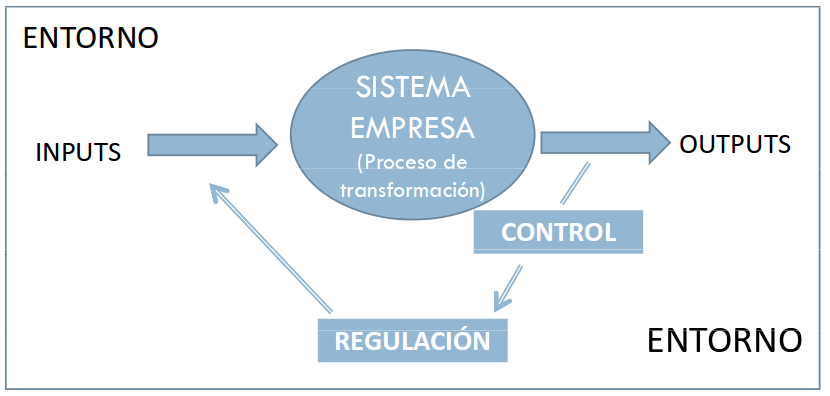
\includegraphics[width=0.8\textwidth]{1}
			 	\caption{La empresa como sistema abierto y autorregulado}
			 	\label{empresa_abierta_regulada}
			 \end{figure}

			Como se aprecia en la \hyperref[empresa_abierta_regulada]{Figura \ref*{empresa_abierta_regulada}}, la empresa está en constante interacción con su entorno, por lo que se considera que un sistema abierto y autorregulado. La empresa influye sobre el entorno y es influida por él. La empresa como sistema abierto está en constante interacción con su medio ambiente y ``logra un equilibrio dinámico, al tiempo que retiene la capacidad para trabajar o transformar energía. La supervivencia del sistema no sería posible sin un proceso continuo de flujo de entrada, transformación y flujo de salida''. En este proceso utiliza unos inputs o factores productivos, como las materias primas, que adquiere a ciertos proveedores o como los recursos humanos del mercado laboral. Una vez finalizado el proceso de transformación, los bienes y/o servicios producidos salen de nuevo al exterior, donde van a ser consumidos. La empresa se relaciona, por tanto, con agentes externos: clientes, proveedores, gobierno, sindicatos, etc.

			Además de mecánico, en tanto que transforma materias primas en productos terminados, el proceso de transformación es también financiero, al transformar ahorro en capital productivo, y mental, porque la empresa procesa información. Igualmente, la empresa necesita disponer de un sistema de control que le permita alcanzar sus objetivos. La falta de control puede conducir al sistema a un estado de estropía, en el que existe un máximo desorden entre los elementos del sistema, lo que puede suponer la desaparición del sistema.

			Se denomina \textbf{retroalimentación} o \textcolor[rgb]{0.5,0.8,0.9}{\textbf{\emph{feedback}}} al mecanismo o sistema de control que permite al sistema conocer si se han producido desviaciones en los límites previamente fijados. Para solucionar estas desviaciones se actuará sobre los inputs para reconducir el sistema a la situación deseada. Además, existe la posibilidad de actuar sobre los propios procesos de transformación a través  del control denominado concurrente. Debido a las razones anteriores, se puede afirmar que la empresa es un sistema autorregulable, pues si se desvía de sus objetivos el proceso de retroalimentación intentará mantener el equilibrio interno obtenido por esa autorregulación, que permite al sistema mantener algunas variables dentro de los límites deseados.

		\section{\textcolor[rgb]{0.5,0.8,0.9}Los subsistemas funcionales de la empresa}
			Una de las ventajas de analizar la empresa como un sistema es que permite abordar su estudio determinando las diferentes partes que la componen. Es el principio de jerarquía de los sistemas el que permite descomponerlos en subsistemas que pertenecen a un sistema mayor. Aun dividiendo los sistemas en partes, cada una de ellas conserva las propiedades del sistema del que deriva.

			El sistema empresa se puede descomponer en diferentes subsistemas. Éstos no deben funcionar aislados sino que deben interactuar para obtener sinergias (situación donde el todo es mayor que la suma de sus partes), logrando ser más productivos que si funcionaran de forma independiente.

			Hay diversas clasificaciones que definen los diferentes subsistemas de la empresa. En nuestro caso, hemos optado por el criterio más extendido, \textbf{el criterio funcional}. Según este criterio, se puede dividir a la empresa en tantos subsistemas como actividades desarrolla. Estos subsistemas serán los siguientes: subsistema de aprovisionamiento, de producción, comercial, financiero, de recursos humanos y de dirección. No todos los subsistemas están presentes en todas las empresas, o, si lo están en ocasiones están integrados en otros subsistemas.

			Las funciones principales de cada subsistema son:
			\begin{description}
				\item[Subsistema de aprovisionamiento], encargado de adquirir los factores necesarios para acometer las actividades de producción; es decir, debe ocuparse de cuestiones relacionadas con la previsión, materialización y gestión de las inversiones de la naturaleza física que se van a incorporar al proceso productivo.

				\item[Subsistema de producción], encargado de la transformación de los inputs en productos o servicios que satisfagan las necesidades del mercado. La producción consiste en el desarrollo de una actividad creadora de bienes y/o servicios encaminados a satisfacer necesidades humanas, de forma que la utilidad de los elementos obtenidos sea superior a la de los empleados para su ejecución. Algunos autores consideran este subsistema como parte del subsistema de aprovisionamiento.

				\item[Subsistema de comercialización], al que compete relacionar la organización con el mercado, desde su conocimiento hasta la distribución de los productos demandados. Actividades comerciales son tanto el aprovisionamiento de inputs como la colocación de outputs; sin embargo, a efectos de subdivisión de la empresa en subsistemas funcionales, se distingue entre el subsistema de aprovisionamiento y el subsistema comercial, también conocido como el subsistema de \textcolor[rgb]{0.5,0.8,0.9}{\emph{marketing}}. Este subsistema se encarga de las decisiones sobre producto, precio, promoción y distribución (conocidas como las ``4 P del marketing mix'': product, price, promotion, place), además de la investigación de mercados.

				\item[Subsistema de recursos humanos], responsable de la administración de los recursos humanos en la empresa. Incluye actividades tales como la planificación de los recursos humanos, para contar en todo momento con el número y tipo de personal que necesita la organización; el reclutamiento de los candidatos más idóneos para los puestos que haya que cubrir; selección de los mejores candidatos a contratar; orientación de los nuevos miembros de la organización; capacitación y desarrollo de los empleados, evaluación del desempeño y retribución.

				\item[Subsistema financiero] (financiación e inversión), encargado de determinar la cuantía de los fondos necesarios para la organización, de suministrarlos y de aplicarlos a las inversiones más convenientes. La misión del subsistema financiero consiste en buscar los fondos necesarios para financiar las actividades empresariales y distribuirlos entre las distintas áreas de la unidad económica o alternativas de inversión. Es el sustento del resto de áreas funcionales, puesto que sin los fondos obtenidos por el mismo sería imposible la realización de cualquier tarea productiva.

				\item[Subsistema de dirección o administrativo o de] \textbf{\textcolor[rgb]{0.5,0.8,0.9}{\emph{management}}}, encargado de la administración de la empresa en sus niveles estratégicos y de gestión. Este subsistema se encarga de la planificiación, organización y control de los subsistemas funcionales velando para que no funcionan de forma independiente persiguiendo sus propios objetivos, sino de forma coordinada persiguiendo los objetivos del sistema empresa. Además, el subsistema de dirección es el encargado de la relación entre la empresa y su entorno, desarrollando una adecuada planificación estratégica que logre proporcionar a la empresa una ventaja competitiva sostenible a largo plazo.
			\end{description}

			En la práctica, no todos estos subsistemas están presentes en la empresa (puede haber más, como el de calidad o menos), ni tienen los mismos nombres. Hay otro subsistema que no ha sido nombrado aquí, pero que está tomando mucha importancia: el subsistema de I+D.

		\section{\textcolor[rgb]{0.5,0.8,0.9}La dirección de empresas: objetivos y funciones generales}
			Los directivos, gestores y administradores son los individuos que dirigen las actividades de una empresa a través de otros. Los desafíos a los que se tienen que enfrentar los directivos son parecidos sea cual sea el sector en el que se encuentren, el tamaño de la empresa o el país en el que ésta esté situada. La dirección de empresas como disciplina de conocimiento trata de analizar los factores que hacen que la gestión que estos directivos desempeñan sea la más adecuada para conseguir el éxito empresarial.

			¿Por qué ciertas empresas obtienen mejores resultados que otras? Para evaluar la actuación de las empresas se tienen en cuenta los resultados de las mismas, es decir, el nivel en la cual la organización logra sus objetivos de forma eficiente y eficaz. La \textbf{eficacia} mide el nivel de cumplimiento que ha logrado una organización respecto a sus objetivos. Si una empresa es eficaz pero no tiene en cuenta los recursos que ha tenido que emplear para lograr dichos objetivos no conseguiría una imagen completa sobre su actuación empresarial. Por ello, es necesario observar el nivel de eficiencia de la empresa. La \textbf{eficiencia} mide si una organización está utilizando la cantidad adecuada de recursos para lograr sus objetivos. Incluso cuando una organización es eficaz puede ser ineficiente. Para lograr un alto desempeño, \underline{las organizaciones deben ser eficientes y eficaces}.

			¿Cuáles son las funciones que llevan a cabo los administradores para lograr la eficiencia y la eficacia? \textbf{Planificación}, \textbf{organización}, \textbf{dirección} y \textbf{control}. Estas funciones son propias del subsistema de dirección.

			En la \textbf{planificación}, los directivos definen los objetivos que se persiguen, se fija la estrategia global para lograr dichos objetivos y se establecen planes que integren y coordinen las actividades de forma coherente.

			Una vez establecida la planificación, los directivos tienen que diseñar una estructura organizativa que incluye las tareas que tienen que realizarse, asignando las personas más idóneas para hacerlas, estableciendo cómo organizar las tareas, quién reporta a quién y dónde se tomarán las decisiones. A esta función se la denomina \textbf{organización}.

			La función de \textbf{dirección} consiste en dirigir y coordinar a los integrantes de la organización.

			Los directivos tienen que asegurarse que las cosas van como deberían ir, vigilando el desempeño de la organización. El desempeño actual debe ser comparado con los objetivos anteriormente planteados. Si existen desviaciones significativas, el trabajo de los directivos será devolver a la organización a la senda establecida. Este proceso de monitorizar, comparar y corregir es lo que denominamos como función de \textbf{control}.

\chapter{\textcolor[rgb]{0.9,0.3,0.3}{El empresario, la dirección y el gobierno de las empresas}}
	\section{\textcolor[rgb]{0.9,0.3,0.3}Evolución histórica del concepto de empresario}
		No es hasta la edad Moderna cuando surge la figura de empresario como sujeto económico, correspondiéndose la misma con el comerciante característico del ``\textcolor[rgb]{0.9,0.3,0.3}{\emph{capitalismo mercantilista}}'', en el que el Estado jugaba un papel prominente en el desarrollo de la actividad económica. Con la Revolución Industrial, la figura del comerciante se sustituyó por la del empresario capitalista. El economista \textbf{Adam Smith} publicó su conocida obra ``\textcolor[rgb]{0.9,0.3,0.3}{\emph{La Riqueza de las Naciones}}'', sentando las bases de la escuela económica del pensamiento clásico, defensora de la libertad de la empresa y contraria al intervencionismo económico estatal.

		Desde la perspectiva de los clásicos, la premisa sobre el funcionamiento automático de los procesos económicos ---la conocida \textcolor[rgb]{0.9,0.3,0.3}{\emph{mano invisible}}--- restaba importancia al alcance de esta figura económica, si bien el empresario cumple el papel primordial de aportar el capital requerido para el funcionamiento del negocio. Por tanto, desde la perspectiva clásica, empresario y capitalista se confunden en la misma persona, configurándose el empresario como \textcolor[rgb]{0.9,0.3,0.3}{\emph{un sujeto de mentalidad económica calculadora racional, fría, sin demasiadas consideraciones de orden moral, humano o social}}.

		Esta visión fría y calculadora, unida a la falta de interés por los problemas humanos y sociales vinculados a las actividades industriales propias de la época, dio lugar a una visión del empresario con claras connotaciones negativas que fueron destacadas por la corriente de pensamiento económico conocida como \textcolor[rgb]{0.9,0.3,0.3}{\emph{Marxismo}} cuyos principales contribuyentes fueron \textbf{Karl Marx} y \textbf{Friedrich Engels} con la obra \textcolor[rgb]{0.9,0.3,0.3}{\emph{El Capital}}. Esta corriente defiende que el origen de la riqueza es el trabajo, y que el beneficio empresarial se deriva de la explotación del factor trabajo. Así, la figura del empresario se equipara a la del capitalista, siendo su función básica la misma que se le atribuía desde la perspectiva clásica: aportar capital.

		Estas dos aportaciones dominaron el mundo económico durante mucho tiempo. Otra aportación importante fue la de \textbf{Richard Cantillon} quien en su obra ``\textcolor[rgb]{0.9,0.3,0.3}{\emph{Ensayo sobre la naturaleza del comercio en general}}'' distingue entre las personas que reciben retribuciones ciertas y las que reciben retribuciones inciertas y asumen los riesgos propios de la actividad económica. Estas últimas personas, \textcolor[rgb]{0.9,0.3,0.3}{\emph{entrepreneurs}}, se definen como agentes que compran medios de producción a un precio dado, para combinarlos en un producto que intentarán vender a un precio incierto que sea superior a sus costes. Así, Cantillon es el primero en caracterizar al empresario como el que asume riesgos en el desarrollo de su actividad económica.

	\section{\textcolor[rgb]{0.9,0.3,0.3}Enfoques sobre la figura del empresario}
		\subsection{\textcolor[rgb]{0.9,0.3,0.3}Teoría del empresario de Knight}
			En esta teoría, el empresario se presenta como un asegurador de las rentas de los factores productivos, a la vez que soporta los riesgos de la actividad económica de la empresa. De esta forma, el beneficio empresarial se justifica como recompensa del riesgo asumido que es inherente a la figura del empresario.

			El empresario adquiere factores productivos a un precio fijado de antemano. Dichos factores se combinarán adecuadamente para obtener los bienes y servicios resultado del desarrollo de la actividad económica y, posteriormente, se ofrecerán al mercado para que sean adquiridos por las personas interesadas (véase \hyperref[empresario_riesgos]{Figura \ref*{empresario_riesgos}})

			\begin{figure}
			 	\centering
			 		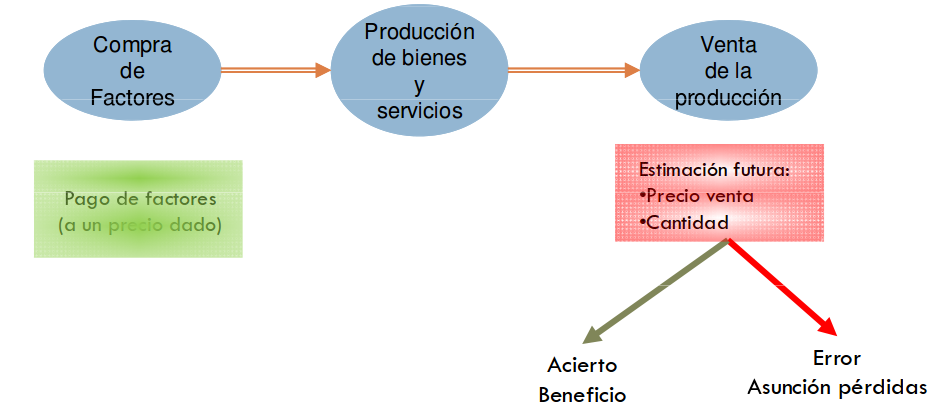
\includegraphics[width=0.8\textwidth]{2}
			 	\caption{El empresario y la asunción de riesgos}
			 	\label{empresario_riesgos}
			 \end{figure}

			 Puesto que el precio de los factores es un coste para el empresario, tanto su cuantía cmo la cantidad de factores a adquirir dependerán de las estimaciones económicas realizadas por el empresario sobre la demanda futura del mercado y los precios de venta de la producción. Si el empresario acierta en sus previsiones, obtendrá un beneficio que compensará la capacidad del empresario para trabajar en un ambiente de incertidumbre controlada\footnote{Cuando se puede determinar la probabilidad de que ocurra un suceso futuro, estamos ante una incertidumbre controlada. Si tal probabilidad no puede ser estimada, estaríamos ante una incertidumbre en sentido puro.}. Si se equivoca, deberá aceptar las pérdidas, pues habrá asumido unos costes superiores a los ingresos derivados de sus ventas.
			 \newpage
			 Los \textbf{riesgos} que asume el empresario son una doble naturaleza:
			 \begin{enumerate}[a)]
			 	\item \textcolor[rgb]{0.9,0.3,0.3}{\emph{Técnicos}}, vinculados a la incertidumbre de llevar a cabo efectivamente la producción esperada y de que los productos se terminen y en las condiciones esperadas por el mercado.
			 	\item \textcolor[rgb]{0.9,0.3,0.3}{\emph{Económicos}}, que tienen que ver con la incertidumbre acerca de que los ingresos derivados de las ventas sean mayores a los costos derivados del aseguramiento de las rentas de los restantes factores que participan en el proceso productivo.
			 \end{enumerate}

			 Aunque algunos autores critican que la actividad empresarial comporta algunos riesgos que son susceptibles de medida y que, por tanto, pueden ser cubiertos, los riesgos típicamente empresariales son difícilmente estimables y asegurables. Es más. Aun cuando tales riesgos fuesen asegurables, la figura del empresario caracterizada por la asunción de riesgos no habría desaparecido, sino que sería el asegurador quien asumiría dicho papel.

		\subsection{\textcolor[rgb]{0.9,0.3,0.3}Teoría del empresario innovador de Schumpeter}
			Según Schumpeter, la naturaleza cíclica e irregular del crecimiento económico se explica por las innovaciones técnicas de los empresarios en un medio competitivo en el que los beneficios no siempre se mantienen. Para Schumpeter, el empresario es un agente central en el desarrollo del sistema capitalista, y el crecimiento económico y el progreso social pueden explicarse a partir del papel que juegan los empresarios en el proceso de cambio tecnológico. (Véase \hyperref[empresario_innovador]{Figura \ref*{empresario_innovador}})

			\begin{figure}
			 	\centering
			 		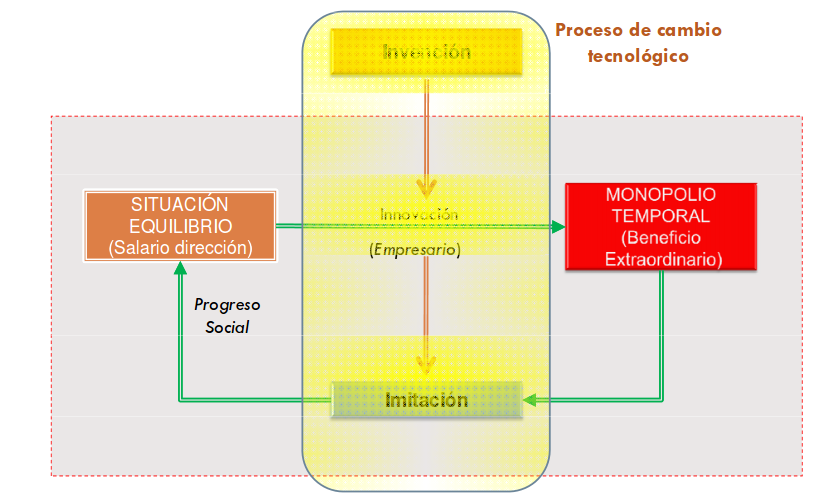
\includegraphics[width=0.8\textwidth]{3}
			 	\caption{Proceso de cambio tecnológico y progreso social}
			 	\label{empresario_innovador}
			 \end{figure}

			 El sistema capitalista tiende a un equilibrio en el que el empresario recibe una retribución por su trabajo---salario de dirección---, lo que constituye un beneficio de naturaleza ordinaria. Sin embargo, el empresario intentará desarrollar innovaciones para romper esta situación de equilibrio y, de tener éxito, el sistema económico pasará a una nueva situación de monopolio en la que el empresario innovador obtendrá beneficios de naturaleza extraordinaria. Esta nueva situación monopolística no es permanente, pues el éxito económico del empresario innovador atraerá la atención de otros empresarios imitadores que, con el tiempo, generalizarán la innovación original y conducirán al sistema económico a una nueva situación de equilibrio caracterizada por un mayor progreso social. Para Schumpeter, este progreso social tiene lugar de manera cíclica y se enmarca dentro de un proceso de ``destrucción creativa''.

			 En el \textbf{proceso de cambio tecnológico} ---eje central del progreso de las economías capitalistas--- cabe distinguir tres fases:
			 \begin{enumerate}[1.]
			 	\item \textcolor[rgb]{0.9,0.3,0.3}{\emph{Invención}}: relacionada con la generación de nuevas ideas; básicamente se corresponde con la creación de un nuevo producto o de un nuevo proceso de producción para un producto ya existente. Esta invención puede tener lugar tanto en el seno de las empresas como fuera de ellas, el autor señala que el empresario no se caracteriza por inventar.
			 	\item \textcolor[rgb]{0.9,0.3,0.3}{\emph{Innovación}}: definida como la aplicación de una invención a nuevos usos industriales y comerciales; abarca distintas acciones, como pueden ser la introducción de un nuevo producto/servicio, la introducción de nuevos procesos productivos\ldots Es necesario considerar que, aparte de innovaciones tecnológicas, pueden existir innovaciones organizativas, comerciales o financieras.
			 	\item \textcolor[rgb]{0.9,0.3,0.3}{\emph{Imitación}}: en la que los empresarios imitadores modifican aspectos no sustanciales de la innovación original, dando lugar a productos y procesos similares.
			 \end{enumerate}

			 Desde la perspectiva de Schumpeter sólo los empresarios innovadores son verdaderos empresarios, si bien hay que reconocer el importante papel que juegan los empresarios imitadores en el proceso de cambio tecnológico, al contribuir a la desaparición de la situación de monopolio y a la generalización de las innovaciones, con el consecuente progreso social. Además, los empresarios imitadores pueden incluir innovaciones de tipo incremental que supongan mejoras en la innovación original; de ahí que no se les pueda negar la etiqueta de empresarios por su contribución al progreso social a través del papel que juegan en el proceso de cambio tecnológico. Sin embargo, en esta teoría la asunción de riesgos no es una característica distintiva del empresario, pues recae sobre los propietarios del capital de la empresa.
		\newpage
		\subsection{\textcolor[rgb]{0.9,0.3,0.3}Teoría de la tecnoestructura de Galbraith}
			Según Galbraith, a lo largo del siglo XX se produjo un proceso de acumulación de capitales que supuso el nacimiento de grandes corporaciones con gran poder. Dichas corporaciones, altamente complejas, no pueden ser dirigidas por una sola persona, de manera que la gestión se reserva a la \textcolor[rgb]{0.9,0.3,0.3}{\emph{tecnoestructura}}, que sería un órgano colegiado que se encarga de dirigir la empresa y que está compuesto por un elevado número de profesionales provenientes de diversos campos del conocimiento.

			Aunque en cierto sentido esta teoría no es realmente una teoría sobre el empresario, en el marco de sus desarrollos teóricos Galbraith defiende una novedosa visión del empresario que supera las propuestas previas en las que el empresario se correspondía con una persona física, proponiendo que el empresario puede estar integrado por varias de estas personas físicas que son profesionales dedicados a la administración de empresas.

			Los planteamientos de Galbraith se basan en la evidencia empírica de un trabajo de Berle y Means. Estos autores demostraron que, a medida que aumentaba el tamaño de las sociedades de capital por acciones, se podía producir una separación entre la propiedad y el control de las empresas. Esta separación se produce porque los accionistas no están interesados en la gestión de la empresa y ceden sus derechos a profesionales de la administración a cambio de recibir una retribución en forma de dividendos por sus aportaciones al capital. En este contexto, la \textcolor[rgb]{0.9,0.3,0.3}{\emph{tecnoestructura}} es realmente la depositaria del poder de las grandes empresas, en cuanto a que marca sus objetivos y toma las decisiones oportunas para alcanzarlos.

	\section{\textcolor[rgb]{0.9,0.3,0.3}Categorías y funciones del empresario: empresario vs. capitalista vs. directivo}
		El paso del tiempo ha alterado la concepción del empresario. Durante largo tiempo el término capitalista fue sinónimo del de empresario, cumpliendo este último la función primordial de aportar el capital requerido para crear la empresa y asegurar el correcto funcionamiento de las organizaciones empresariales. Con los años, diversas teorías sobre el empresario vinieron a distinguir la función propia del capitalista de la otras dos figuras con atributos diferenciados: empresario\footnote{También se acuña el término de emprendedor, especialmente como agente innovador que identifica y explota nuevas oportunidades con la creación de nuevas empresas o en empresas ya existentes} y directivo.

		Según Cuervo y Montoro, mientras que el empresario se caracteriza por buscar nuevas oportunidades de negocio que permitan obtener beneficios explotando situaciones que incitan al cambio, los directivos son encargados de supervisar el proceso de combinación de recursos de producción y distribución, siendo la labor de los directivos especialmente relevante cuando las empresas no operan con la máxima eficiencia. Dentro de la categoría de empresario se distinguen dos perfiles:
		\begin{enumerate}[a)]
			\item El \textbf{empresario individual propietario}, figura que se correspondería con la visión clásica del empresario como persona física, en la que coincidirían las figuras del empresario y del capitalista y a la que serían de aplicación los rasgos característicos desarrollados en la presentación de la teoría del empresario innovador y el empresario riesgo.

			\item El \textbf{empresario corporativo}, para hacer referencia al empresario que, sin participación significativa en el capital de la empresa, la controla. Esta visión estaría más próxima a las propuestas de la \textcolor[rgb]{0.9,0.3,0.3}{\emph{tecnoestructura}}.
		\end{enumerate}

		\begin{center}
			\textbf{Empresarios, capitalistas y directivos}
			\begin{tabular}{|>{\columncolor[rgb]{0.9,0.3,0.3}}l | l | l | l |}
				\hline
				\rowcolor[rgb]{0.9,0.3,0.3} & \textbf{Empresario} & \textbf{Capitalista} & \textbf{Directivo} \\
				\hline
				\textbf{Caracte-} & - Descubre y explota & - proprietario del & - Administra y \\
				\textbf{izado por} & oportunidades & capital: accionistas & gestiona recursos \\
				& - Un creador, que inicia & - Accionistas & - Un administrador \\
				& motiva el proceso & de control & \\
				& de cambio & - Accionista pasivo & \\
				\hline
				\textbf{compor-} & - Acepta el riesgo & - Aversión al riesgo & - Aversión al riesgo \\
				\textbf{tamiento}& - Intuición, alerta, & - Evalúa alternativas & - Decisor ``racional'' \\
				& exploración & - Elección de activos & - Crear y mantener \\
				& - Liderazgo y ruptura en & de riesgo & ventaja competitiva \\
				& los nodos de actuación & & - Crear confianza para \\
				& - Identifica oportunidades & & la cooperación \\
				& de negocio & & - Supervisión del \\
				& - Creación de empresas & & proceso administrativo \\
				\hline
			\end{tabular}
		\end{center}

	\section{\textcolor[rgb]{0.9,0.3,0.3}La estructura de propiedad de la empresa}
		La propiedad de la empresa se relaciona con la participación en el capital requerido para la creación y funcionamiento de la empresa, de manera que todo partícipe en dicho capital tiene la consideración legal de ``propietario''.

		Según el profesor Bueno, la estructura de propiedad de una empresa se relaciona con el modo en que se distribuye el capital entre los diferentes propietarios. La concentración mayor o menor del capital dará origen a la existencia de uno o varios grupos de propiedad que pueden ser clasificados tal y como se muestran en la siguiente tabla:
		\begin{center}
			\textbf{Grupos de propiedad en la empresa}
			\begin{tabular}{| c | c | c |}
				\hline
				& Particulares y & Residentes \\ \cline{3-3}
				& familias & No residentes \\ \cline{2-3}
				Sector privado & Empresas industriales y &  Nacionales \\ \cline{3-3}
				& de servicios (capital empresarial) & Extranjeras \\ \cline{2-3}
				& Entidades financieras & Nacionales \\ \cline {3-3}
				& (capital bancario) & Extranjeras \\
				\hline
				\multicolumn{3}{|l|}{Sector público} \\
				\hline
			\end{tabular}
		\end{center}

		Estas categorías de propiedad pueden mostrar diferencias en cuanto a los objetivos perseguidos. Mientras que algunos propietarios persiguen obtener una rentabilidad rápida de sus inversiones, para otros es más importante controlar la empresa, y sus objetivos de rentabilidad se establecen en con un plazo temporal más largo. Es por esto que al hablar de los accionistas de una empresa debemos distinguir entre \textbf{accionistas de control} y \textbf{accionistas pasivos}.

		La estructura de propiedad puede diferir de una empresa a otra, de un sector de actividad a otro e incluso, de un país a otro.

	\section{\textcolor[rgb]{0.9,0.3,0.3}La dirección: función y niveles}
		\subsection{\textcolor[rgb]{0.9,0.3,0.3}Dirección y gobierno de la empresa}
			La propiedad de una empresa conlleva derechos y obligaciones tanto de contenido económico como jurídico. En el devenir diario de una empresa hay directivos que toman decisiones que afectan a su funcionamiento y que no tienen por qué ser titulares de su capital. Estos directivos supervisan el proceso de combinación de recursos productivos que vienen fijados en las empresas, para aumentar la eficiencia y alcanzar los objetivos que vienen fijados por el empresario.

			Cuestionándonos quiénes son los propietarios de las empresas y quiénes las dirigen, en el caso de las personas físicas es fácil identificar al propietario de la empresa con la persona física que desarrolla la actividad empresarial y que se encarga de dirigir su empresa. Sin embargo, dentro de las sociedades de capital podemos encontrar situaciones que van desde el caso en el que existe un solo propietario hasta otros en los que existen miles.

			Por tanto, asumiendo que es posible la separación entre la propiedad y la dirección, deberíamos preguntarnos cómo es posible garantizar que los responsables de dirigir las mismas no adoptarán decisiones que vayan en contra de los intereses de los propietarios o de otros grupos de interés. 

			Cuando las personas encargadas de la dirección son además los únicos propietarios la cuestión queda resuelta de forma automática, pues quien ejerce la dirección es también propietario y no adoptará decisiones que vayan en contra de sus intereses como titular del capital. No obstante, en aquellas situaciones en las que los responsables de la dirección de la empresa no son propietarios, deben arbitrarse mecanismos que permitan compatibilizar los objetivos de los directivos y propietarios, surgiendo el concepto de gobierno corporativo. El gobierno de la empresa se relaciona con el conjunto de mecanismos de control implantados para evitar que los directivos puedan tener comportamientos que vayan en contra de los objetivos de los propietarios o de otros grupos que pueden tener intereses en la empresa.

		\subsection{\textcolor[rgb]{0.9,0.3,0.3}Niveles de dirección}
			\begin{description}
				\item[La alta dirección] está formada por personas con responsabilidad sobre toda la empresa y de las que depende su éxito o fracaso. Sus funciones básicas pasan por fijar los grandes objetivos y estrategias que deberán alcanzarse en el largo plazo por la empresa. Representan el papel del empresario. Ocupan el estrato superior de la jerarquía. Aquí se incluiría el ejecutivo de la empresa, que lo formaría el director ejecutivo (consejero delegado o CEO ---\textcolor[rgb]{0.9,0.3,0.3}{\emph{Chief Executive Officer}}---), junto con todos aquellos que él considere que participan en los procesos de análisis de generación de alternativas y elección de las principales decisiones de la empresa.

				\item[La dirección media] formada por los directivos de una escala inferior. Son responsables de desarrollar las decisiones que se han tomado en el nivel superior en relación a su área de responsabilidad y en coordinación con las demás. Establecen objetivos a medio y corto plazo, planifican y controlan las acciones para su logro, y organizan y dirigen a las personas que tienen que llevarlas a cabo. Son el enlace jerárquico para la transmisión de las decisiones desde los niveles más altos a los más bajos.

				\item[La dirección de primera línea] está constituida por los supervisores de primera línea, encargados del seguimiento diario de los empleados que realizan las actividades propias del objeto de la empresa. Su principal responsabilidad es garantizar que se cumplen los objetivos que les vienen designados por el nivel superior.
			\end{description}

			Aunque las actividades de planificación, organización, dirección y control son ejercidas por todos los niveles de dirección, el tiempo dedicado a ellas depende del lugar ocupado en la jerarquía. En los directivos de alto nivel predominan las dos primeras, a medida que la dirección se ejerce en niveles más bajos, las funciones que ocupan más tiempo son las de dirección y control.
	
	\section{\textcolor[rgb]{0.9,0.3,0.3}El gobierno de la empresa}
		\subsection{\textcolor[rgb]{0.9,0.3,0.3}Concepto de gobierno corportativo}
			El Gobierno Corporativo es la definición de la relación entre los inversores, accionistas y directivos. Ante la evidencia de que las rentas suelen ser capturadas por los colectivos con mayor poder negociador, se deben establecer criterios para una distribución equitativa de la riqueza entre los propietarios de los recursos y para asegurar una adecuada entrega de valor al sistema en el que se mueven las organizaciones. 

			Esta relación se puede establecer a través de la \textcolor[rgb]{0.9,0.3,0.3}{\emph{teoría de los skateholders}}, que considera que el éxito empresarial se consigue cuando la gesión está orientada a las partes interesadas o \textcolor[rgb]{0.9,0.3,0.3}{\emph{skateholders}} y se han establecido las oportunas vías de diálogo. En un contexto de información asimétrica surgen conflictos entre las partes interesadas, que pueden pretender apropiarse de los excedentes del negocio. Por ello, el gobierno corporativo debe crear una estructura eficiente de incentivos y responsabilidades que impidan que ciertos colectivos usen y abusen de la información privilegiada de la que dispongan.

			Se trata por tanto de que a través de los códigos de buen gobierno se delimiten estas estructuras y relaciones, de forma tal que la gestión conjunta de impactos sociales, medioambientales y económicos, propios de la gestión con criterios de responsabilidad social corporativa\footnote{comprimiso continuo que deben adoptar las empresas para contribuir al desarrollo económico sostenible, trabajando con los empleados, sus familias, la comunidad local y la sociedad, en general, para mejorar su calidad de vida.} (RSC), se realice con la completa y plena aceptación de los propietarios y directivos de las empresas. De esta forma se estará gobernando con criterios de transparencia informativa y de relación con los distintos grupos de interés. Este sería el punto de conexión entre el gobierno corporativo y la responsabilidad social corporativa, y también el punto de partida de un nuevo estilo empresarial de dirección en el que su rendimiento y continuidad no estén basadas exclusivamente en la disciplina de una organización jerárquica, lo que hará posible la delegación de responsabilidad y que la ``renta de capital'' no sea el único objetivo de la empresa.

		\subsection{\textcolor[rgb]{0.9,0.3,0.3}Mecanismos de control}
			Aunque hay distintos modelos de gobierno corporativo, dependiendo de variables endógenas como la estructura o la actividad de la empresa, o de variables exógenas como las circunstancias históricas, culturales o económicas de los países, todos ellos tienen su principal punto de diferenciación en los mecanismos de control existentes. Mediantes estos mecanismos se dirigen y controlan las empresas, y pueden clasificarse en dos amplias categorías, según sean internos (diseñados por la propia organización) o externos (diseñados por el mercado).

			\subsubsection*{\textcolor[rgb]{0.9,0.3,0.3}Mecanismos internos}
				Actúan en forma preventiva, intentando evitar riesgos y garantizando, en la medida de lo posible, el logro de los objetivos organizacionales. Son desplegados y operados por grupos de interés internos, y sus efectos deben abarcar a todos los actores involucrados en una organización.

				\begin{description}
					\item[Junta General]: La Junta General es un órgano necesario que expresa con sus acuerdos, adoptados por mayoría, la voluntad social. Ante todo es una reunión de accionistas no permanente. No está dotado de poderes ommímodos para decidir válidamente toda clase de asuntos. Por ejemplo, no puede adoptar acuerdos contrarios a los estatutos. Aunque sí tiene la potestad de nombrar a los administradores y de impartir instrucciones al órgano de administración. Para llevar a cabo el cambio de los miembros del consejo, en el caso de disconformidad con su actuación, se han de destinar recursos para analizar las actividades del mismo, que no todos los accionistas están dispuestos a soportar. En muchos casos, cuando la empresa está cotizada, muchos optan por vender sus acciones en vez de analizar estas deficiencias. Lo normal es que sean los accionistas más importantes los que realicen dicha tarea.

					\item[Órganos de Administración]: En las sociedades de capital, los órganos de administración son los que ejercen la gestión y representación de las mismas. Por tanto, son necesarios y permanentes. Conforme al artículo 210 de la nueva Ley, la administración de la sociedad se podrá encomendar a un administrador único, a varios que actúen de forma solidaria o a un consejo de administración. Por tanto, se trata de un conjunto de personas elegidas por los accionistas para administrar y representar la sociedad y también para supervisar al equipo directivo y ratificar sus decisiones más importantes.
				\end{description}

				\subsubsection{\textcolor[rgb]{0.9,0.3,0.3}Mecanismos externos}
					Son mecanismos que limitan la capacidad de los directivos para mantener comportamientos oportunistas. Actúan de forma preventiva y correctiva, y su existencia evita riesgos y contribuye a que todos los objetivos organizativos se alcancen.
					\begin{description}
						\item[Tomas de control hostiles]: la regulación legal de este mecanismo, denominado Oferta Pública de  Adquisición de Valores, tiene un doble objetivo: favorecer las operaciones que aumenten la riqueza general de una economía y establecer los mecanismos que aseguren el reparto de las rentas generadas por la operación según el ideal de equidad de la sociedad. La búsqueda de ambos objetivos afectará a la capacidad de financiación de las empresas y a la transferencia en el funcionamiento del gobierno corporativo de las compañías. La finalidad de la normativa sobre la OPA es controlar como se producen los cambios en la dirección de una empresa. Entre las razones para efectuar un cambio de control estarían las específicas del oferente y la ineficiencia de los gestores de la empresa. Son mecanismos de control muy potentes, que normalmente ocurren cuando se tienen pobres resultados en una compañía por una gestión incorrecta. En estos casos, la compra y el cambio de administración suele mejorar los resultados y obtener un elevado beneficio.

						\item[Mercados financieros y estructura financiera de la empresa]: Una buena gestión de la estructura financiera de la empresa permite el acceso a financiación en mejores condiciones, lo que lleva aparejada una mejora en los resultados y en las previsiones de futuro. Esto afecta positivamente a la reputación de los directivos y facilita el logro de los objetivos de los accionistas. El cumplimiento de los objetivos económicos es señal para los mercados financieros que facilitan el logro de financiación en condiciones más beneficiosas para la empresa. También la estructura financiera de la empresa afecta a su valor. Si el capital de la misma se obtiene a través del endeudamiento  externo, se reducirán los fondos de libre disposición, pues parte de ellos se deberán destinar al pago de intereses y a devolver el principal del préstamo. De esta forma, la relación entre deuda y recursos propios (estructura financiera) afectará al valor de la empresa. Sin embargo, si la financiación se hace a través de la emisión de participaciones (acciones), no se establecerá ningún tipo de interés en el contrato, y la remuneración de los accionistas se hará una vez pagados el resto de compromisos, lo cual no afectará a la estructura financiera de la compañia.

						\item[Mercado laboral de consejeros y directivos]: La alta competencia en el mercado laboral de consejeros y directivos es una forma de asegurar el correcto funcionamiento de las organizaciones, pues sólo podrán mantener sus puestos de trabajo o podrán promocionar profesionalmente aquellos que desempeñen correctamente sus funciones maximizando el valor para los accionistas. Así, los directivos desarrollarán su labor basándose en buenas prácticas y construyendo una reputación positiva con el objetivo de mantener su puesto de trabajo o promocionar a mejores puestos directivos.
					\end{description}
	\section{\textcolor[rgb]{0.9,0.3,0.3}Modelos de gobierno corporativo}
		\subsection{\textcolor[rgb]{0.9,0.3,0.3}Modelo anglosajón}
			Se caracteriza por un accionariado disperso. Es el que se sigue en EEUU y Gran Bretaña.

			Las empresas suelen ser más independientes al no estar controladas por un grupo reducido de accionistas. También suele ser importante la presencia de inversores institucionales. Por eso, en este modelo la transferencia de la propiedad y el control de las compañías se suele hacer a través de OPAs. En estos países suele estar bastante desarrollada la transparencia informativa, los Códigos de Buen Gobierno, los derechos de los accionistas minoritarios y las normas sobre OPAs. El inconveniente de este modelo es que los inversores se preocupan por la rentabilidad a corto plazo antes que por la viabilidad de la empresa.

		\subsection{\textcolor[rgb]{0.9,0.3,0.3}Modelo alemán}
			Es el modelo continental europeo, con modelos propios en cada uno de los países, a excepción de Gran Bretaña. La concentración accionarial es muy importante y las empresas suelen estar controladas por grupos de inversores estables con participaciones cruzadas y con un importante protagonismo en la gestión de la organización, lo que hace aumentar los blindajes y el obstáculo a las OPAs.

			En este modelo los accionistas minoritarios tienen una escasa protección, por lo que corren auténtico riesgo de que sustraigan las rentas que les pertenecen. Y su sistema de gestión es dual, pues normalmente tienen un consejo de administración encargado de la dirección y gestión, y un consejo de supervisión, con funciones de control, en el que suelen estar representados los trabajadores juntos a los accionistas más importantes.

		\subsection{\textcolor[rgb]{0.9,0.3,0.3}Modelo japonés}
			Su sistema es monista, estando dominado por directivos con importantes participaciones accionariales cruzadas entre empresas. El típico consejo está compuesto por 21 miembros, casi todo empleados de la empresa. El presidente del consejo suele ser el primer ejecutivo, que junto a dos o tres directivos más tiene derechos especiales para representar la compañía.

\chapter{\textcolor[rgb]{0.3,0.6,0.4}{Objetivos, planificación y control}}
	\section{\textcolor[rgb]{0.3,0.6,0.4}La planificación de la empresa: concepto y tipos de planes}
		La planificación empresarial comprende todas aquellas acciones gerenciales dirigidas a determinar los objetivos futuros y medios más apropiados para lograrlos, lo que va a suponer escoger entre distintos cursos de acción. Esta función administrativa comprende un conjunto de etapas a realizar de forma secuencial, que persiguen contestar a las preguntas de hacia dónde queremos ir y cómo podemos llegar. Hay que vincular un horizonte temporal ya que si no es ambigüo, en los planes también se específica de qué manera se van a perseguir los objetivos.

		La planificación va a facilitar el correcto desarrollo de las otras tres funciones gerenciales, siendo en muchos casos un punto de partida para sus respectivas puestas en marcha. Además, la planificación aporta ciertos beneficios:
		\begin{enumerate}[-]
			\item Permite la coordinación de esfuerzos. Una de las principales funciones de los gerentes es coordinar el trabajo de los individuos y de los grupos. Una forma de lograr este objetivo es determinar los objetivos globales de la organización, así como los objetivos específicos de cada parte, en consonancia con los primeros, de tal manera que el esfuerzo se dirija hacia la consecución de ambos.

			\item Facilita la preparación para el cambio, ya que delinea un futuro deseado y la forma para conseguirlo.

			\item Permite el desarrollo de estándares de rendimiento.

			\item Facilita el desarrollo de los gerentes, que desarrollan habilidades de toma de decisiones.
		\end{enumerate}

		La planificación es la base para decidir el tipo de estructura a adoptar por la empresa, el perfil de los trabajadores a contratar, el estilo de liderazgo, etc.

		La planificación será eficaz si reúne los siguientes requisitos:
		\begin{enumerate}[1.]
			\item \textcolor[rgb]{0.3,0.6,0.4}{\textbf{\emph{Unidad}}}: más de un plan para alcanzar la misma meta puede provocar confusión.

			\item \textcolor[rgb]{0.3,0.6,0.4}{\textbf{\emph{Continuidad}}}: la planificación es un proceso secuencial.

			\item \textcolor[rgb]{0.3,0.6,0.4}{\textbf{\emph{Precisión}}}: ha de aprovecharse al máximo la información posible para planificar de forma correcta.

			\item \textcolor[rgb]{0.3,0.6,0.4}{\textbf{\emph{Flexibilidad}}}: los planes deben alterarse y cambiarse; no deben ser estáticos, porque el entorno cambia.
		\end{enumerate}

		\begin{figure}
			 	\centering
			 		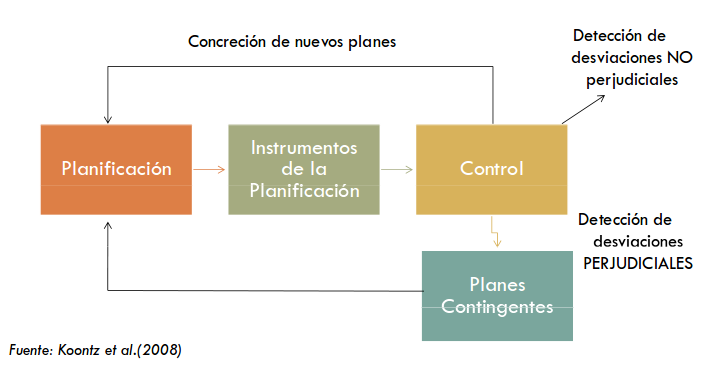
\includegraphics[width=0.9\textwidth]{4}
			 	\caption{Relaciones entre la planificación y el control}
			 	\label{plan_control}
		 \end{figure}

		La planificación requiere que los gerentes tomen decisiones relativas a un conjunto de elementos propios de esta función, que se desarrollan de forma interrelacionada:

		\begin{enumerate}[1.]
			\item Los \textbf{objetivos}: concretan las situaciones futuras que una empresa espera alcanzar en un horizonte temporal o determinado.

			\item Las \textbf{acciones}: son los medios, actividades o cursos de acción definidos para alcanzar los objetivos.

			\item Los \textbf{recursos}: van a determinar qué curso de acción es el más adecuado, ya que un plan implica determinar qué cantidad y calidad de recursos requiere y cómo deben asignarse éstos. En función de los recursos que tengamos podemos determinar unas acciones u otras o según las acciones que vayamos a hacer, podemos determinar que necesitamos unos recursos u otros.

			\item La \textbf{implantación}: se refiere a la determinación de los medios y las formas de ejecutar los distintos cursos de acción.

			\item El \textbf{control}: establecer mecanismos que detecten las desviaciones que se produzcan respecto a lo planificado. En la \hyperref[plan_control]{Figura \ref*{plan_control}} se esquematiza la relación entre planificación y control. El control es necesario para que la planificación llegue a un fin determinado. 
		\end{enumerate}

	\section{\textcolor[rgb]{0.3,0.6,0.4}Etapas de la planificación}
		La planificación empresarial suele contemplar un conjunto de etapas, tal y como se visualiza en la \hyperref[planificacion]{Figura \ref*{planificacion}}.

		\begin{figure}
			 	\centering
			 		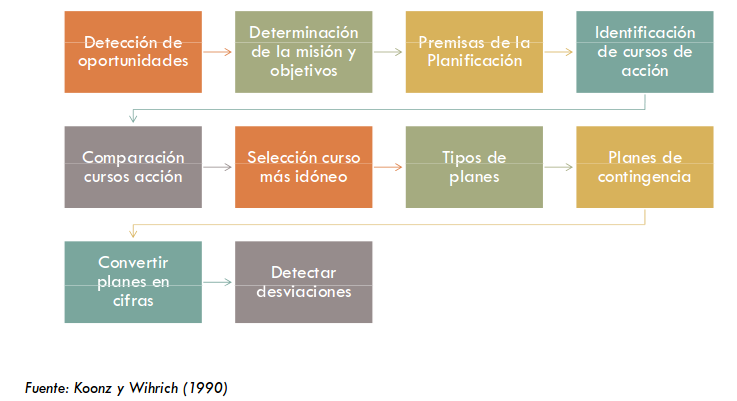
\includegraphics[width=0.9\textwidth]{5}
			 	\caption{Etapas de la función de planificación}
			 	\label{planificacion}
		\end{figure}

		Así, en un primer momento, se debe analizar la información existente tanto en el interior como en el exterior de la empresa, determinando las amenazas, oportunidades(análisis externo), debilidades y fortalezas (análisis interno). En definitiva, la empresa debe hacer un análisis DAFO (deblidades, amenazas, fortalezas y oportunidades).

		A continuación, una vez concretada esa meta a largo plazo que es la \textbf{misión}, se deben especificar los objetivos a alcanzar por la organización.

		El siguiente paso en esta secuencia es establecer premisas de la planificación, esto es, determinar pronósticos acerca del entorno donde el plan debe desarrollarse. Así, podremos conocer en qué condiciones internas o externas operarán nuestros planes.

		Para alcanzar las metas, se debe identificar, comparar y finalmente seleccionar el curso de acción más adecuado para la empresa en función de sus recursos, entre todas las alternativas que se hayan propuesto.

		Es habitual que la planificación no sea exacta, por lo que deberá contemplarse el diseño de planes de contingencia o de apoyo, que apoyen y complementen la planificación básica. Estos planes pueden prever todo tipo de contingencias, como por ejemplo, planes para comprar equipos o materias prima extra.

		Finalmente, para poder establecer los mecanismos de detección de desviaciones sobre lo planificado es necesario cuantificar los planes. Tenemos que encontrar el punto en todo la planificación en el que retomar dicha planificación y conseguir nuestros objetivos.
	\newpage
	\section{\textcolor[rgb]{0.3,0.6,0.4}Tipología de planes}
		Se pueden distinguir dos grandes grupos de planes: planes estratégicos y planes operativos.

		\begin{center}
			\textbf{Características de los planes estratégicos y planes operativos}
			\begin{tabular}{|p{4.7cm}|p{4.7cm}|p{4.7cm}|}
				\hline
				\rowcolor[rgb]{0.3,0.6,0.4} \textbf{Dimensiones} & \textbf{Planes estratégicos} & \textbf{Planes operativos} \\
				\hline
				Concepto & Plasman los objetivos a largo plazo de la empresa & Interpretan los planes estratégicos para que sean desarrollados en el día a día de la empresa \\
				\hline			
				Horizonte temporal & Largo plazo & Corto plazo \\
				\hline
				Alcance & Todas las actividades de la empresa & Actividades concretas de la empresa \\
				\hline
				Nivel de alcance & Menor & Mayor \\
				\hline
				Dependencia & No dependen de otro plan & Dependen de los planes estratégicos, puesto que los instrumentalizan \\
				\hline
			\end{tabular}
		\end{center}

		Los planes operativos pueden ser clasificados en planes de un solo uso o planes permanentes. Los primeros hacen referencia a las actuaciones de carácter no rutinario que se desarrollan en la organización, mientras que los planes permanentes comprenden todas aquellas actividades rutinarias que se emprenden. 

		Los \textbf{planes permanentes} más empleados son las políticas, los procedimientos y las reglas (ordenado según nivel de concreción, de más general a menos). Las \textbf{políticas} son declaraciones que guían y canalizan el pensamiento ante la toma de decisiones, reflejan la filosofía de la empresa. Definen el marco de actuación dentro del que se puede tomar una decisión, de tal forma que será consistente con los objetivos de la empresa. Las políticas cumplen tres propósitos fundamentales:
		\begin{enumerate}[-]
			\item Asegurar que las decisiones tomadas serán consistentes con las metas.

			\item Asegurar una consistencia en la forma de proceder en la toma de decisiones.

			\item Facilitar la delegación de autoridad, conservando el control sobre lo que los subordinados hagan.
		\end{enumerate}

		Los \textbf{procedimientos} son guías para la acción, recogen las instrucciones detalladas para ejecutar acciones que se presentan con regularidad en la empresa. Su relación con las políticas es muy estrecha, ya que los procedimientos permiten su ejecución y van en línea con ellas, no podemos poner un procedimiento de reclamación que vaya en contra de la política de reclamaciones.

		Las \textbf{reglas} establecen situaciones específicas, pueden o no llevarse a cabo, no admitiendo discrecionalidad alguna (a diferencia de las políticas). Los procedimientos están constituidos por un conjunto de reglas; sin embargo, una regla puede o no pertenecer a un procedimiento.

		Respecto de los \textbf{planes de uso único}, los más conocidos son los programas y los presupuestos. Los \textbf{programas} contienen un conjunto de especificaciones sobre responsabilidades, recursos, datos temporales y otros elementos necesarios para poder realizar un determinado curso de acción, una vez ejecutado un programa ya no vale para ser ejecutado de nuevo, ya que está pensado para una tarea determinada. Un \textbf{presupuesto} es un plan ``cuantificado'', es decir, detalla los resultados esperados en términos numéricos, ya sea en términos financieros, de horas laborales, etc. Al expresar en una medida numérica un plan, se está convirtiendo automáticamente es un instrumento de control.

	\section{\textcolor[rgb]{0.3,0.6,0.4}Los peligros de la planificación: paradojas}
		La función de planificación se ve envuelta en una serie de paradojas que pueden dificultar su efectividad:
		\begin{enumerate}[1.]
			\item La planificación requiere de la incertidumbre del entorno, ya que si la empresa dispusiera de información veraz y completa sobre cómo va a evolucionar éste, no haría falta planificar, ya que las decisiones de la empresa serían siempre acertadas. Sin embargo, si la incertidumbre es elevada, lo planificado pierde su validez y puede conducir a la empresa a tomar decisiones irreales e incoherentes con los cambios producidos en el entorno.

			\item La toma de decisiones irreales también puede venir provocada por la extremada precisión con la que se formulen objetivos y planes, siendo esta precisión un elemento necesario para el correcto desarrollo de esta función, ya que estaríamos encorsetando nuestro plan, esto se conoce como parálisis por análisis.

			\item La planificación implica asignar recursos escasos a los distintos planes. Cuanto mayor sea el horizonte temporal de la planificación, más tiempo estarán comprometidos dichos recursos, siendo la planificación más inflexible.

			\item La planificación deriva en problemas de coordinación en muchos casos, ya que establece un marco de actuación donde es especifica qué se debe hacer, quién lo ejecutará y cuando.
		\end{enumerate}
		
	\section{\textcolor[rgb]{0.3,0.6,0.4}Los objetivos de la empresa: concepto y tipología}
		La \textbf{misión} de la empresa es el propósito básico que quiere alcanzar la organización, debe tener vocación de largo plazo. No se debe confundir este concepto con la \textbf{visión}, que es el enunciado de la situación futura ideal de la empresa. Tampoco se debe confundir con el \textbf{eslogan}, que es sólo un instrumento publicitario claro, consiso y que identifica a la empresa en la sociedad, la palabra ``eslogan'' viene de ``slogan'' (grito de guerra).

		Los \textbf{objetivos} son los fines hacia los que se dirige la actividad empresarial, deben cumplir los siguientes atributos:
		\begin{enumerate}[1.  ]
			\item Ser \textcolor[rgb]{0.3,0.6,0.4}{\textbf{\emph{mensurables}}}: venir expresados en una unidad numérica y un horizonte temporal delimitado.

			\item Ser \textcolor[rgb]{0.3,0.6,0.4}{\textbf{\emph{realizables}}}: deben ser objetivos realistas, consistentes con la calidad y cantidad de los recursos humanosm tecnológicos y financieros de la empresa.

			\item Ser \textcolor[rgb]{0.3,0.6,0.4}{\textbf{\emph{flexibles}}}: los objetivos deben estar definidos de tal forma que se facilite y garantice su adaptación a las condiciones cambiantes del entorno.

			\item Ser \textcolor[rgb]{0.3,0.6,0.4}{\textbf{\emph{comprensibles}}}: para alcanzar un objetivo, todo esfuerzo empresarial debe dirigirse hacia su consecución, por lo que es imprescindible la comunicación de éste a todos los niveles de la empresa. La comunicación será más ágil y la interpretación del objetivo se garantizará cuanto más sencillo de entender sea éste.
		\end{enumerate}

		Existen tres grandes grupos de objetivos: la misión de la empresa, los objetivos estratégicos y los operativos. De los primeros emana toda la empresa, los segundos hacen referencia a los fines que pretende alcanzar la empresa en el largo plazo, mientras que los terceros guiarán las actividades que deben realizarse en el día a día. Es normal que en la empresa existan multiplicidad de objetivos. Para saber la importancia relativa de cada objetivo podemos analizar la \hyperref[jerarquia_objetivos]{Figura \ref*{jerarquia_objetivos}}.

		\begin{figure}
			 	\centering
			 		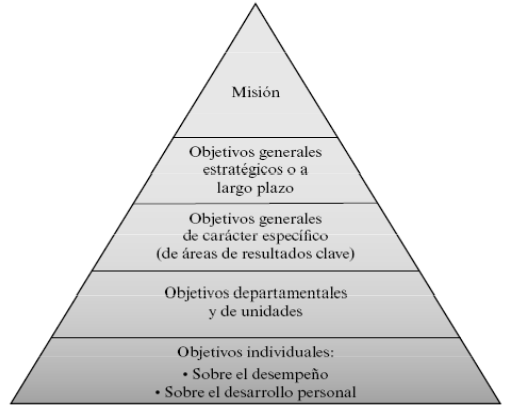
\includegraphics[width=0.7\textwidth]{6}
			 	\caption{Jerarquía de objetivos en una organización}
			 	\label{jerarquia_objetivos}
		\end{figure}
		
	\section{\textcolor[rgb]{0.3,0.6,0.4}El control de la empresa}
		El control es la función administrativa que permite evaluar el desempeño de las acciones emprendidas en el seno de la empresa. Es decir, establecer mecanismos de control en una empresa significa poner en marcha un conjunto de procesos que verifiquen si las actividades realizadas han conseguido alcanzar las metas previamente planteadas, definiendo para el caso de que no se adecúen, medidas correctivas de las desviaciones producidas.

		El control se desarrollará a través de un conjunto de etapas de carácter secuencial. Así, un sistema de control típico tendrá cuatro grandes etapas: establecer los estándares de rendimiento, medir el desempeño, comparar estándares y desempeño con objeto de determinar las desviaciones que se hayan producido y tomar medidas correctivas que reconfiguren las actividades desviadas o refuercen las actividades exitosas. La \hyperref[proceso_control]{Figura \ref*{proceso_control}} resume este proceso.

		\begin{figure}
			 	\centering
			 		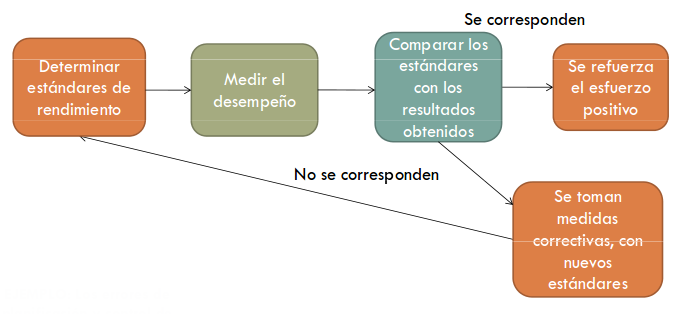
\includegraphics[width=0.9\textwidth]{7}
			 	\caption{El proceso básico de control}
			 	\label{proceso_control}
		\end{figure}

		\subsection{\textcolor[rgb]{0.3,0.6,0.4}Tipos de control}
			\begin{description}
				\item[Control preliminar]: en vez de esperar a los resultados de las actuaciones emprendidas, los gestores pueden  ejercer control limitando las actividades, esto es, evitando los problemas antes de que se produzcan. Este tipo de control pretende, antes de que en la empresa se inicien las actividades, garantizar que éstas se llevarán a cabo de la forma más correcta posible.

				\item[Control concurrente]: este tipo de control actúa cuando los planes se están ejecutando, dirigiendo y supervisando las actividades conforme se están llevando a cabo. Gracias a los nuevos avances de la Tecnología de la Informacióon y la Computación el control concurrente es una de las herramientas más potentes para evaluar el desempeño.

				\item[Control de retroalimentación]: los administradores emplean los resultados obtenidos en acciones anteriores para ir adaptando y corrigiendo las desviaciones que surjan en las actividades actuales respecto de los estándares establecidos.
			\end{description}

			Para que los sistemas de control sean efectivos, deben diseñarse siguiendo una serie de requisitos:
			\begin{enumerate}[-]
				\item Determinar estándares de rendimiento realistas y válidos.
				\item Establecer un sistema de comunicación eficaz en todos los niveles de la empresa, facilitando la retroalimentación.
				\item Conseguir que todos los miembros de la empresa conozcan y acepten el sistema de control empleado.
				\item Motivar que los empleados comuniquen inmediatamente cualquier desviación detectada.
			\end{enumerate}

	\section{\textcolor[rgb]{0.3,0.6,0.4}Sistemas de planificación y control}
		\subsection{\textcolor[rgb]{0.3,0.6,0.4}Administración por objetivos}
			La administración por objetivos (APO) es un sistema formal diseñado para evaluar el progreso de gerentes y subordinados en el cumplimiento de metas. Dispone de un conjunto de procedimientos que guían como deben establecerse los objetivos y metas, y evalúan el desarrollo de las operaciones así como el desempeño final que éstas han obtenido.

			La APO incluye tres estapas específicas:
			\begin{enumerate}[1.]
				\item \textcolor[rgb]{0.3,0.6,0.4}{\emph{Se fijan metas y objetivos específicos en cada nivel de la organización.}}
				\item \textcolor[rgb]{0.3,0.6,0.4}{\emph{Los gerentes y subordinados fijan juntos las metas de éstos últimos.}}
				\item \textcolor[rgb]{0.3,0.6,0.4}{\emph{Los gerentes y sus subordinados revisan periódicamente el avance logrado hacia las metas de éstos últimos.}}
			\end{enumerate}

			Para que la APO funcione y sea eficaz, gerentes y empleados deben estar convencidos de que las evaluaciones del desempeño son justas, válidas y equitativas. Por tanto, serán determinantes las habilidades para el liderazgom la motivación y la delegación de autoridad de los gerentes.

		\subsection{\textcolor[rgb]{0.3,0.6,0.4}Cuadro de Mando Integral}
			Un Cuadro de Mando Integral (CMI) es un formato objetivo para describir las principales actividades de una empresa mediante una serie de medidas enfocadas a cuatro grandes perspectivas: financiera, de cliente, del proceso y del desarrollo (véase \hyperref[mando_integral]{Figura \ref*{mando_integral}}).

			\begin{figure}
			 	\centering
			 		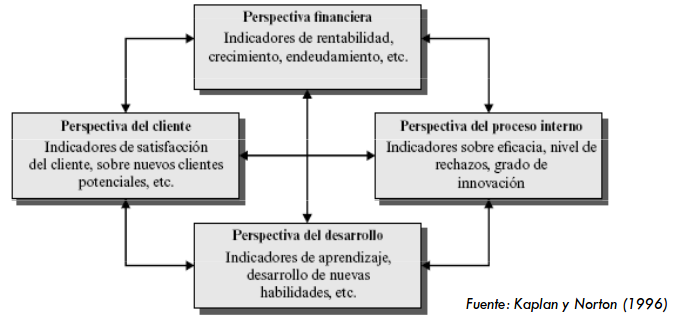
\includegraphics[width=0.9\textwidth]{8}
			 	\caption{Cuadro de Mando Integral Básico}
			 	\label{mando_integral}
			\end{figure}

			Las cuatro grandes perspectivas en las que se centra son:
			\begin{description}
				\item[Financiera]: se centra en los aspectos financieros y en el valor que genera la empresa para sus accionistas.
				\item[Cliente]: está orientada a valorar las relaciones de la empresa con sus clientes, así como las expectativas futuras que los consumidores tendrán sobre la organización.
				\item[Procesos internos]: analiza si los procesos internos de la empresa son adecuados.
				\item[Desarrollo de las personas y el aprendizaje]: está enfocada a valorar cómo se gestionan los empleados y si existe una cultura que motive el aprendizaje.
			\end{description}

			Por tanto, un CMI es un formato genérico fácil de entender que sirve para describir los objetivos y logros de una empresa. Es una herramienta útil para:
			\begin{enumerate}
				\item Comunicar estrategias planificadas a todos los niveles de la empresa.
				\item Discutir aquellas actividades motivadas por metas estratégicas.
				\item Supervisar y recompensar actividades.
			\end{enumerate}

\chapter{\textcolor[rgb]{0.5,0.1,0.4}{La Función de Organización}}
	\section{\textcolor[rgb]{0.5,0.1,0.4}Introducción}
		La función de organización tiene por objeto la creación de una estructura organizativa que permita aprovechar eficaz y eficientemente los recursos con los que cuenta una organización.

		El diseño de la estructura organizativa es el resultado de un conjunto de decisiones que los directivos irán tomando con el fin de conseguir una adecuada utilización y coordinación de los recursos. Estas decisiones irán configurando lo que se denomina dimensión vertical y horizontal de la organización. Dichas decisiones se verán condicionadas por algunos factores sobre los que la organización tiene poco o nulo control. Estos factores se denominan \textcolor[rgb]{0.5,0.1,0.4}{\emph{factores de contingencia}}. Finalmente, la estructura organizativa resultante del proceso de diseño organizativo tendrá un efecto muy importante sobre el desempeño organizativo.

	\section{\textcolor[rgb]{0.5,0.1,0.4}Diseño Organizativo}
		Se denomina \emph{\textcolor[rgb]{0.5,0.1,0.4}{diseño organizativo}} al proceso por medio del cual los administradores crean la estructura de la organización bajo los criterios de eficacia y eficiencia.

		La \textbf{estructura} de una organización se puede definir como la forma de agrupar las diferentes tareas a realizar y las realizaciones que se producen por la ejecución total de la actividad de la empresa.

		La estructura se representa gráficamente a través de un \textbf{organigrama}, que muestra las relaciones jerárquicas y de asesoría entre los departamentos y unidades en los que se han agrupado los diferentes puestos de trabajo. La ventaja principal de esta representación es la clarificación de las relaciones formales dentro de la organización, evitando así conflictos entre las personas o unidades que no tienen claras sus posiciones.

		La estructura ideada y planteada por la empresa es denominada \textcolor[rgb]{0.5,0.1,0.4}{\emph{estructura formal}}. Coexiste con la \textcolor[rgb]{0.5,0.1,0.4}{\emph{estructura informal}}, conformada por las relaciones no formales que surgen de manera espontánea y se crean como resultados de las actividades e interacciones entre los individuos integrantes de la organización. Esta estructura informal está basada en los vínculos afectivos de los miembros de la organización y da lugar a redes sociales dentro de la propia organización. Tanto la estructura formal como la informal componen la estructura real de la organización.

		\subsection{\textcolor[rgb]{0.5,0.1,0.4}Partes de la organización y mecanismos de coordinación según Mintzberg}
			\begin{figure}
			 	\centering
			 		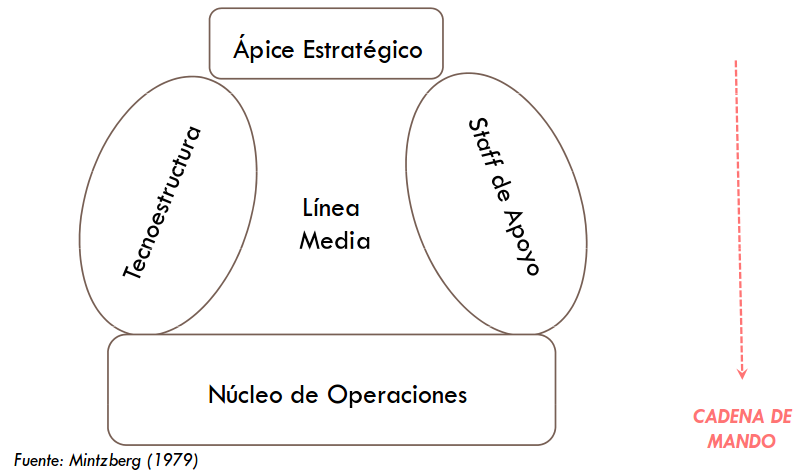
\includegraphics[width=0.9\textwidth]{9}
			 	\caption{Partes de la organización según Mintzberg}
			 	\label{organizacion_mintz}
			\end{figure}
			La organización consta de cinco partes fundamentales (como muestra la \hyperref[organizacion_mintz]{Figura \ref*{organizacion_mintz}}):
			\begin{description} 
				\item[Ápice estratégico]: Lo conforma la alta dirección, que se encarga de establecer los objetivos generales y diseñar y desarrollar la estrategia para conseguirlos. Actúa como vínculo entre la empresa y el entorno.

				\item[Núcleo de operaciones]: Compuesto por trabajadores (operarios), encargados de realizar las actividades y tareas directamente relacionadas con la producción de los productos/servicios que constituyen el negocio de la organización (flujo de operaciones). Cumplen las siguientes labores:
				\begin{enumerate}
					\item Asegurar las materias primas (\textcolor[rgb]{0.5,0.1,0.4}{\emph{inputs}}) necesarias para la producción (\textcolor[rgb]{0.5,0.1,0.4}{\emph{output}}).

					\item Transformación de las materias primas en los productos finales.

					\item Distribución de los \textcolor[rgb]{0.5,0.1,0.4}{\emph{outputs}}.

					\item Y demás funciones relacionadas directamente con las anteriores.
				\end{enumerate}

				\item[Línea media]: engloba a todos los directivos que conectan jerárquicamente el ápice estratégico con el núcleo de operaciones. Su principal misión es servir de vínculo entre estas dos partes de la organización. Además, recoge información sobre el desempeño de su propia unidad, transmite una parte de ésta a los niveles jerárquicos superiores y se encarga de formular la estrategia de su unidad.

				\item[Staff de apoyo]: Contiene unidades que realizan actividades de apoyo que no pertenecen al flujo de operaciones (mantenimiento, seguridad, cafetería, etc.)

				\item[Tecnoestructura]: formada por unidades de analistas cuya misión fundamental es diseñar y planificar o cambiar el trabajo de otras partes de la organización, además de formar o enseñar a otros trabajadores a realizar su trabajo. También sirven de analistas, estudiando el entorno y controlando el resto de actividades de la organización. Al igual que el \textcolor[rgb]{0.5,0.1,0.4}{\emph{staff}} de apoyo esta parte de la organización queda fuera del flujo de operaciones.
			\end{description}
			Mintzberg también propone la existencia de cinco mecanismos de coordinación:
			\begin{description}
				\item[Adaptación mutua]: la coordinación se logra mediante la comunicación entre empleados. Esta forma de comunicación es más habitual en organizaciones pequeñas y simples, pero también en las complicadas, para resolver problemas.

				\item[Supervisión directa]: Una persona coordina el trabajo, dando instrucciones u órdenes a otros y supervisando sus acciones.

				\item[Normalización de los procesos de trabajo]: Se consigue especificando los procesos y tareas a realizar, mediante normas, reglas y procedimientos que establecen cómo ha de realizarse el trabajo.

				\item[Normalización de los resultados]: Se establecen los resultados que deben ser obtenidos en la realización del trabajo.

				\item[Normalización de habilidades]: Se consigue detallando las habilidades o destrezas requeridas para desarrollar el trabajo.
			\end{description}

		\subsection{\textcolor[rgb]{0.5,0.1,0.4}Pasos del diseño organizativo}
			La existencia del diseño organizativo radica en la división del tranajo, según la cual algunas tareas son subdivididas en actividades más pequeñas o sencillas que son asignadas a los trabajadores para su ejecución. Esta división del trabajo es la que conduce a la creación de puestos de trabajo, a la agrupación de éstos en departamentos, a la coordinación interna de dichos departamentos y a la coordinación entre los diferentes departamentos. 

			La secuencia lógica del diseño organizativo sería la siguiente:
			\begin{enumerate}[1.]
				\item Establecimiento de los objetivos y planes de la organización (realizado en la etapa de planificación).
				\item Identificación y clasificación de las actividades necesarias para alcanzar los objetivos de la organización.
				\item Agrupación de las actividades en puestos de trabajo individuales.
				\item Agrupación de los puestos en funciones o divisiones (departamentalización de la organización).
				\item Asignación de administradores a todas y cada una de las diferentes unidades anteriormente creadas.
				\item Establecimiento de mecanismos de coordinación horizontal y vertical de la estructura.
			\end{enumerate}

	\section{\textcolor[rgb]{0.5,0.1,0.4}Dimensiones del diseño organizativo}
		Cuando los directivos se enfrentan al diseño de una estructura organizativa, éstos deben atender a las dimensiones vertical y horizontal de la misma. La dimensión vertical tiene en cuenta todo el conjunto de relaciones que surgirán entre los diferentes niveles jerárquicos existentes dentro de la organización. Por el contrario, la dimensión horizontal se encarga de analizar el conjunto de relaciones que existen entre las unidades que hay dentro de un mismo nivel.

		\subsection{\textcolor[rgb]{0.5,0.1,0.4}Dimensión vertical}
			La dimensión vertical comprende todo el conjunto de decisiones que afectan al número de niveles jerárquicos y las relaciones entre ellos. En la medida en que el número de niveles sea muy elevado, nos encontramos con estructuras denominadas altas. Por el contrario, estructuras con un número de niveles reducido se denominan planas. Las \textbf{estructuras altas} son estructuras con una mayor complejidad vertical, mientras que las \textbf{estructuras planas} presentan un mayor nivel de complejidad horizontal.

			Con respecto a la dimensión vertical, hay que conocer los siguientes conceptos que se ven afectados por las decisiones de los administradores:
			\subsubsection{\textcolor[rgb]{0.5,0.1,0.4}Unidad de mando}
				El principio de la unidad de mando expresa que cada subordinado debe tener un solo supervisor. Un subordinado con varios supervisores podría dar lugar a numerosos conflictos, pues el subordinado no sabría a quién atender en caso de recibir órdenes contradictorias de diferentes jefes.

			\subsubsection{\textcolor[rgb]{0.5,0.1,0.4}Autoridad y responsabilidad}
				La autoridad es un derecho legítimo de una posición para timar decisiones que afectan a otros, es decir, dar órdenes y esperar su cumplimiento. La autoridad reside en los puestos más que en las personas, por lo que una vez que una persona abandona un puesto ésta pierde la autoridad inherente al mismo. La existencia de diferentes grados de autoridad determina la existencia de diferentes niveles jerárquicos, constituyendo la pirámide organizacional (más poder en la cúspide y menos poder a medida que se desciende por la misma). Surge así el concepto de jerarquía de autoridad de la organización, la cual puede ser definida como la relación entre los diferentes niveles de autoridad en la que los superiores mandan sobre los subordinados.

				El concepto de autoridad no debe ser confundido con el de \emph{\textcolor[rgb]{0.5,0.1,0.4}{poder}}, consistente en la capacidad para influir en las creencias o acciones de otros.

				Muy vinculado al concepto de autoridad se encuentra el de \textcolor[rgb]{0.5,0.1,0.4}{\emph{responsabilidad}}, consistente en la obligación de cumplir con las órdenes recibidas o tareas asignadas.

			\subsubsection{\textcolor[rgb]{0.5,0.1,0.4}Intervalo, tramo o ámbito de control}
				El proceso de creación de departamentos da lugar a la designación de un supervisor de los diferentes miembros que componen la unidad. La cuestión que emerge es saber cuántos subordinados debe tener a su cargo la persona responsable de una unidad organizativa. Así pues, por \emph{\textcolor[rgb]{0.5,0.1,0.4}{tramo de control}} se entiende el número de subordinados que un responsable de departamento puede supervisar eficaz y eficientemente. No podemos establecer un número extacto de subordinados, pues el ejercicio de una supervisión eficaz y eficiente dependerá de diversos factores como el tipo de tecnología utilizada, las habilidades del directivo, etc.

				Los tramos de control podrán ser más amplios cuando:
				\begin{enumerate}
					\item Los puestos de trabajo están definidos con claridad y exentos de ambigüedad.
					\item Existe una alta capacitación por parte de los subordinados.
					\item Existe una alta capacitación por parte del supervisor.
					\item Los subordinados demandan a los supervisores autonomía en la ejecución de su trabajo.
					\item Los puestos de trabajo se encuentran normalizados.
				\end{enumerate}

				El tramo de control con el que cuente la empresa determina el número de niveles que presentará la misma, de tal modo que las organizaciones con tramos de control estrechos dan lugar a estructuras altas, mientras que las organizaciones con tramos de control amplios dan lugar a estructuras planas. 

				Las estructuras altas presentan algunas ventajas, como son un mayor control, supervisión y comunicación entre supervisor y subordinado, debido al escaso número de éstos. Entre los inconvenientes se podría indicar que es una estructura económicamente más costosa. También resulta ser una estructura donde surgen dificultades de comunicación entre la cima y la base, por la mayor longitud de los canales de comunicación. Las estructuras altas son más complejas verticalmente, pues presentan más niveles y exigen una mayor coordinación entre los mismos.

				Las estructuras planas tienen algunas ventajas, como la existencia de delegación por parte de los administradores en los subordinados, lo que les confiere a estos últimos una mayor autonomía en el desarrollo de su trabajo. Además, son estrucuras económicamente menos costosas. Como inconveniente, se puede indicar que puede surgir una sobrecarga del trabajo en los supervisores. Las estructuras planas son estructuras más sencillas verticalmente, con menos niveles y más fácil coordinación entre ellos.

			\subsubsection{\textcolor[rgb]{0.5,0.1,0.4}Centralización vs descentralización}
				Los conceptos centralización y descentralización están asociados al grado de concentración o dispersión de autoridad para la toma de decisiones. Las organizaciones, en sus orígenes, suelen tener la capacidad de decisión concentrada en la cúspide. Esto es lo que se denomina \textcolor[rgb]{0.5,0.1,0.4}{\emph{centralización de la autoridad}}. Sin embargo, a medida que las organizaciones aumentan su tamaño y complejidad necesitan que la alta dirección pueda concentrarse en otras actividades, por lo que necesitan dispersar la autoridad para la toma de decisiones en diferentes partes de la organización. Este proceso de delegación de autoridad de los niveles superiores a los inferiores de denomina descentralización.

				El proceso de descentralización no es un proceso arbitrario, sino que busca delegar la toma de decisiones en las personas que tienen un conocimiento más próximo del problema, y en aquellos puntos de la organización en los que dichas personas se ven afectadas más directamente. Este aspecto resulta especialmente revelante cuando la organización se encuentra en un entorno que cambia rápidamente, lo que exige que las decisiones tengan que ser adoptadas de forma clara.

				Las ventajas de la descentralización son:
				\begin{enumerate}
					\item Dota a la organización y sus trabajadores de una mayor flexibilidad para actuar frente a los cambios del entorno.
					\item Libera a la alta dirección de parte de la toma de decisiones, permitiéndole concentrarse en otros aspectos de la estrategia organizativa.
					\item Favorece la autonomía de los trabajadores, con la consiguiente motivación para los mismos.
				\end{enumerate}
				Por otro lado, entre las desventajas encontramos:
				\begin{enumerate}
					\item Demasiada autoridad por parte de las unidades organizativas o departamentos podría provocan que fueran en contra de las metas organizacionales.
					\item Pueden darse problemas de comunicación y coordinación entre funciones y divisiones.
					\item Dificulta el establecimiento de una política uniforme.
					\item Puede dar lugar a pérdidas de control por parte de los administradores de más alto nivel.
				\end{enumerate}

				Se dice que los puestos de trabajo están especializados verticalmente cuando la capacidad de decisión reside en el supervisor. Cuando se hace una delegación de autoridad en el subordinado, hablamos de la existencia de un puesto de trabajo ampliado horizontalmente.

		\subsection{\textcolor[rgb]{0.5,0.1,0.4}Dimensión horizontal}
			La construcción de la dimensión horizontal de la estructura organizativa se apoya en la división del trabajo y en la posterior agrupación de puestos de trabajos.

			\subsubsection{\textcolor[rgb]{0.5,0.1,0.4}División del trabajo}
				La división del trabajo es el proceso mediante el cual una tarea o actividad es fraccionada en varias subtareas y cada una es realizada por un individuo diferente. Asociados a la división del trabajo están los conceptos de especialización o ampliación del puesto de trabajo. Se dice que los puestos de trabajo están especializados horizontalmente cuando éstos desarrollan pocas tareas o con poco contenido. Entre las razones existentes para especializar horizontalmente los puestos de trabajo se encuentra el aumentar la productividad a través del efecto aprendizaje.

				Lo contrario de la especialización horizontal del puesto de trabajo es la ampliación horizontal, que consiste en aumentar el número de tareas diferentes que un puesto determinado ha de realizar. Se puede reducir la monotonía derivada de la existencia de un número reducido de tareas para así aumentar la motivación por parte de los subordinados.

				El resto está en conseguir que los puestos de trabajo sean eficaces y eficientes, y la clave está en determinar el número de tareas que serán asignadas a cada puesto. Así pues, el procedimiento es el siguiente: analizar todas las tareas que deben realizarse, y después diseñar los puestos que mejor permitan a la organización cumplir con sus objetivos.

				Al finalizar el proceso de diseño de puestos de trabajo, la organización debe conseguir una buena descripción de todos y cada uno de los puestos, la cual debe contener como mínimo:
				\begin{enumerate}
					\item Una relación de todas las actividades que hay que realizar
					\item Cuál es la función básica de cada puesto.
					\item Cuáles son los resultados más importantes a obtener.
					\item Cuál es la autoridad de posición y la responsabilidad asociada.
				\end{enumerate}

			\subsubsection{\textcolor[rgb]{0.5,0.1,0.4}Departamentalización}
				Los departamentos surgen como consecuencia de la necesaria agrupación de actividades y personas bajo un supervisor que los coordine y se responsabilice de ellos. Se define un departamento como un área específica de una organización sobre la cual un administrador tiene autoridad para el desempeño de las actividaeds establecidas.

				La existencia de diferentes criterios utilizados por los administradores para realizar estas agrupaciones da lugar a la existencia de diferentes tipos de departamentalización. No hay una agrupación mejor que otra, pues cada una presenta sus ventajas y desventajas. Las agrupaciones más habituales son:
				\begin{description}
					\item[Departamentalización por función o funcional]: Consiste en agrupar personas que trabajan juntas y poseen habilidades similares o usan los mismos tipos de conocimientos o herramientas para desempeñar su trabajo, dando como resultado agrupaciones vinculadas a las funciones básicas de la empresa. Es de las más utilizadas por las organizaciones.

					\item[Departamentalización geográfica]: Consiste en la agrupación de las actividades y personas de un área o territorio bajo la dirección de un directivo. Este tipo de agrupación suele encontrarse en aquellas organizaciones que operan en áreas geográficas muy amplias. La razón de esta departamentalización se debe a la dificultad que encuentran los responsables funcionales para gestionar los asuntos que surgen en zonas geográficas distintas, con problemáticas específicas. En algunos casos se observa que las necesidades de los clientes varían de una región a otra por lo que este tipo de agrupación permite a los directivos atender a dichas necesidades de una mejor manera.

					\item[Departamentalización por clientes]: Consiste en la agrupación de actividades y personas bajo el interés común de los diferentes tipos de clientes. Tiene como objetivo facilitar la adaptación de los productos y servicios a las necesidades concretas de cada tipo de cliente, logrando así una toma de decisiones más flexible y adaptada a las necesidades cambiantes de los clientes.

					\item[Departamentalización por productos]: Consiste en la agrupación de actividades y personas sobre la base de la existencia de diferentes productos. Permite que el responsable de una línea de producto adquiera la visión global, así como la autoridad y responsabilidad de la misma. Suele ser habitual cuando las empresas crecen en tamaño.

					\item[Agrupaciones híbridas]: Las organizaciones no utilizan un único criterio de departamentalización, sino que diversos criterios se pueden combinar a lo largo de la estructura organizativa.
				\end{description}

	\section{\textcolor[rgb]{0.5,0.1,0.4}Factores de contingencia}
		En el diseño organizativo de una empresa hay que tener en cuenta ciertos parámetros o factores que van a afectar o condicionar su efectividad, los \textcolor[rgb]{0.5,0.1,0.4}{\emph{factores de contingencia}}. Los más importantes son:
		\subsection*{\textcolor[rgb]{0.5,0.1,0.4}Edad}
			La edad de las organizaciones generalmente afecta a la estructura organizativa. Las organizaciones más antiguas tienden a formalizar su comportamiento institucionalizando las relaciones que se producen en su seno y los canales de comunicación. Con la experiencia, muchos aspectos pasan de ser inciertos a ser predecibles, por lo que suelen utilizar reglas para responder a estas circunstancias predecibles. Este mayor establecimiento de reglas lleva a una mayor formalización e institunacionalización. También, a mayor edad de las organizaciones, éstas suelen aumentar la especialización horizontal de trabajo, con el objetivo de lograr mayor eficiencia. Todo ello hace que también se creen más niveles o eslabones para supervisar y coordinar que se cumplen todas estas reglas y protocolos. En consecuencia, las empresas son más conservadoras, menos creativas y menos flexibles. La organización debe intentar equilibrar la necesidad de control y consistencia en sus operaciones con la necesidad de flexibilidad y creatividad, para poder adaptarse rápidamente a los cambios.

		\subsection*{\textcolor[rgb]{0.5,0.1,0.4}Tamaño}
			Este factor tiene efectos similares a la edad. Además, hay que considerar que las organizaciones tienen a crecer a medida que pasa el tiempo, por tanto, a mayor edad, mayor tamaño. Las organizaciones más grandes suelen tener una estructura más compleja, una especialización horizontal más acentuada, mayor número de departamentos y un componente administrativo más desarrollado. Estos departamentos más diferenciados son más fáciles de supervisar, permitiendo un mayor tramo de control.

		\subsection*{\textcolor[rgb]{0.5,0.1,0.4}Tecnología}
			La tecnología engloba las herramientas, maquinaria, sistemas de información, etc. que la organización utiliza para complementar las tareas y actividades que se engloban en su seno. Para analizar la influencia de este factor en la estructura de la organización, Mintzberg se basó en dos dimensiones de la tecnología, la regulación y la sotisficación:
			\begin{description}
				\item[Dimensión reguladora]: Indica el grado en el que el trabajo es controlado por el sistema técnico. Cuando el sistema técnico es muy regulador es fácil establecer las tareas, al venir establecidas por el sistema técnico, provocando la especialización del trabajo y, con ello, mayor formalización de los procesos.

				\item[Sotisficación]: Grado de dificultad para entender el funcionamiento del sistema técnico. No debe confundirse con la dificultad de uso. La sotisficación se refiere a la dificultad en la adquisión de conocimientos o habilidades necesarias para idear, diseñar o reparar el sistema técnico. Cuando un sistema técnico es muy sotisficado, se necesitan expertos más técnicos para su diseño, modificación y reparación, los cuales están o pertenecen a las unidades de apoyo. Como consecuencia, cuanto más sotisficado es el sistema técnico se necesitan más y mayores unidades de apoyo de naturaleza profesional cuyo funcionamiento requiere un mayor nivel de descentralización.
			\end{description}

		\subsection*{\textcolor[rgb]{0.5,0.1,0.4}Entorno}
			Las características del entorno condicionan muchas de las actuaciones de la empresa, y la estructura organizativa no es una excepción.

			Cuando la empresa se enfrenta a un entorno muy \textbf{dinámico} no puede prever lo que ocurrirá, por lo que el establecimiento de normas y reglas no son de mucha utilidad práctica.  Por eso, cuanto más dinámico es el entorno de una organización, la estructura de ésta será más orgánica\footnote{Se puede considerar como el extremo opuesto de la estructura burocrática, y, por tanto, es una estructura poco formalizada/normalizada.} Asimismo, cuando el entorno es estable es más fácil estandarizar las actividades estableciendo reglas.

			Si el entorno es \textbf{complejo} (diíficil de entender), son necesarios una gran variedad de conocimientos y habilidades. Por tanto, la toma de decisiones no puede ser llevada por una sola persona o por miembros de la alta dirección. Es conveniente delegar la autoridad en los subordinados con los conocimientos y habilidades necesarias, de manera que la estructura de la organización ante entornos complejos se descentraliza.

			Sin embargo, si el entorno es \textbf{hostil} (supone una amenaza o daño) de forma súbita, la organización tiene que responder de una forma rápida y a corto plazo, y para ello lo mejor es centrarlizar las decisiones.

	\section{\textcolor[rgb]{0.5,0.1,0.4}Formas organizativas}
		\subsection{\textcolor[rgb]{0.5,0.1,0.4}Funcional}
			Esta forma organizativa agrupa los puestos de trabajo en unidades según las funciones básicas de la empresa\footnote{Actividades necesarias para el funcionamiento de la operativa de una organización}, como producción, marketing, finanzas, etc.

			Los trabajadores en cada departamento se especializan en las mismas actividades. Por ello, su formación procede de áreas de conocimiento asociadas con cada función y comparten, generalmente, las mismas habilidades, usando los mismos equipamientos.

			Estas unidades altamente especializadas requieren una planificación común, por lo que la alta dirección asume gran parte de las decisiones.

			Esta especialización presenta algunas ventajas:
			\begin{enumerate}
				\item Facilita la coordinación y comunicación dentro de cada unidad, debido a que sus miembros comparten los mismos conocimientos básicos, lenguaje y perspectivas.

				\item Ofrece sinergias de aprendizaje y experiencia y, con ello, economías de escala. Esta forma organizativa es más eficiente cuando la organización produce pocos productos o líneas de productos estándares en grandes volúmenes. Por eso, una organización con una estructura funcional es adecuada en un entorno simple y estable.
			\end{enumerate}
			Aunque también supone las siguientes desventajas:
			\begin{enumerate}
				\item Dificulta la coordinación entre los diferentes departamentos.
				\item La centralización de la toma de decisiones hace el proceso de decisión mñas lento y reduce la facilidad de la organización de adaptarse a nuevas circunstancias o a un entorno dinámico.
				\item Son necesarios un mayor número de niveles jerárquicos, además, las actividades requieren una integración mas completa de las principales funciones.
			\end{enumerate}

		\subsection{\textcolor[rgb]{0.5,0.1,0.4}Divisional}
			Cuando la organización crece y empieza a producir una gama más amplia de bienes y servicios para diferentes clases de clientes, pueden surgir varios problemas que reducen la eficiencia y la eficacia de la estructura funcional. En este momento, surgen otras agrupaciones alternativas, como son la agrupación geográfica, por clientes o por producto.

			Estas tres agrupaciones son realizadas atendiendo a criterio de mercado y surgen para dar respuesta a las necesidades de los clientes. Estas formas de agrupación son conocidas como el \textcolor[rgb]{0.5,0.1,0.4}{\emph{enfoque divisional}} o \textcolor[rgb]{0.5,0.1,0.4}{\emph{estructuras divisionales}}. Esta forma divisional agrupa departamentos en base a núcleos de negocio estratégicos de la empresa.

			Estas unidades se consideran divisiones autónomas, pues deben tomar decisiones referentes a su unidad de negocio específica. Por su parte, la sede central delimita la estrategia central de la empresa y conserva una serie de funciones que proporciona de forma centralizada. Así asigna recursos para cada una de las divisiones y recolecta los beneficios.

			La principal ventaja es su potencial de adaptación a las exigencias del mercado. Aunque uno de los principales inconvenientes es la duplicación de funciones en cada división, reduciendo las sinergias y las economías de escala. Además, este tipo de estructura es tendente a generar conflictos entre las divisiones.

			En conclusión, la forma divisional es adecuada cuando la empresa quiere diversificar su mercado. La casi autonomía de sus divisiones le permite responder a los cambios del entorno de forma más rápida, por lo que no precisa de un entorno estable para su desarrollo.

		\subsection{\textcolor[rgb]{0.5,0.1,0.4}Matricial}
			La forma matricial combina dos o más variables en un mismo nivel jerárquico para realizar la agrupación de tareas en departamentos. Habitualmente, una de las variables de agrupación es funcional y la otra está basada en las unidades de negocio.

			Esta forma organizacional se originó con la intención de aprovechar las ventajas de las estructuras funcional y divisional al mismo tiempo.

			Este tipo de estructura permite que trabajadores con formaciones funcionales diferentes participen en los mismos proyectos. Así, se intenta aprovechar las sinergias funcionales y se evita la competencia entre diferentes proyectos.

			La principal característica de esta forma organizacional es la ruptura del principio de unidad de mando. Esto puede generar conflicto de órdenes o prioridades y dar lugar a disfunciones.

			Este diseño permite a la organización ser flexible, permitiéndole actuar en entornos complejos y dinámicos.

\end{document}